

\documentclass[12pt,oneside, a4paper]{book}

\usepackage{etex}
\usepackage{xcolor}
\usepackage[pdftex]{graphicx}
\usepackage{rotating}
\usepackage{epsfig}
\usepackage{epstopdf}
\usepackage[T1]{fontenc}
\usepackage[utf8]{inputenc}
\usepackage{cmap}
\usepackage[croatian]{babel}
\usepackage[unicode]{hyperref}
\usepackage{mathptmx}
\usepackage{amscd}
\usepackage{amssymb}
\usepackage{amsmath}
\usepackage{amsfonts}
\usepackage[left=2.5cm,right=2.5cm,top=2.5cm,bottom=2.5cm]{geometry}
\usepackage{setspace} 
\usepackage{hhline}
\usepackage{enumerate}
\usepackage{delarray}
\usepackage{array}  
\usepackage{tabularx} 
\usepackage{multirow}  
\usepackage[bf, font=small]{caption}
\usepackage[labelfont=small, font=small]{subcaption}
\usepackage{wasysym}
\usepackage{subeqnarray}
\usepackage{pdflscape} % setting page into landscape view
\usepackage{enumitem} % for itemize lists
\usepackage[toc,page]{appendix}
\newcommand{\HRule}{\rule{\linewidth}{0.5mm}}
\usepackage{makeidx}
\usepackage{nomencl}
\usepackage{listings}
\lstset{basicstyle=\ttfamily,breaklines=true}
\usepackage{courier}
% Podesavanje izgleda zaglavlja i podnozja strana
\usepackage{fancyhdr} 
\usepackage{titlesec}
\usepackage{float}
\usepackage{url}
\def\UrlBreaks{\do\/\do-}

\titleformat{\chapter}{\normalfont\huge\bfseries}{\thechapter\bfseries.}{20pt}{\huge\bfseries}

\fancypagestyle{plain}{%
  \fancyhf{}% Clear header/footer
  \fancyfoot[OR]{{\thepage}}%
  \fancyfoot[EL]{{\thepage}}%
  \renewcommand{\headrulewidth}{0pt}%
}

% required for printing index
% use \index{name} in text
%\usepackage{makeidx}
%\makeindex
% required for printing nomenclature
% use \nomenclature{symbol}{description} in text
%\usepackage{nomencl}
%\makenomenclature
%\renewcommand{\nomname}{Popis oznaka}




%Opcionalno
%\linespread{1.3}
%\setlist{nolistsep}   % setting for itemize lists
%\renewcommand{\thefootnote}{\fnsymbol{footnote}}  % to get unnumbered footnotes

% Adding a dot after chapter number in TOC 
%\let\savenumberline\numberline
%\def\numberline#1{\savenumberline{#1.}}



%\pagestyle{fancyplain}


%\rfoot{\thepage}
% iskljucivanje broja strane iz Sadrzaja, Popisa slika i Popisa tabela
\AtBeginDocument{\addtocontents{toc}{\protect\thispagestyle{empty}}}
\AtBeginDocument{\addtocontents{lof}{\protect\thispagestyle{empty}}}
\AtBeginDocument{\addtocontents{lot}{\protect\thispagestyle{empty}}}

%\rhead{\slshape \nouppercase \leftmark}
%\lhead{} %delete left header


%Podesavanje izgleda referenci
\usepackage[square, numbers, sort]{natbib} 


% Bibliography u "Literatura"
\addto\captionscroatian{%
  \renewcommand{\bibname}{Literatura}
  \renewcommand{\tablename}{Tabela}
  \renewcommand{\nomname}{Popis oznaka}
  \renewcommand{\indexname}{Indeks pojmova}
  \renewcommand{\lstlistingname}{Program}
}
%"Popis tablica" u "Popis tabela"
\addto\captionscroatian{\renewcommand{\listtablename}{Popis tabela}}
\addto\captionscroatian{\renewcommand\appendixname{Prilog}}
\addto\captionscroatian{\renewcommand\appendixpagename{Prilozi}}
\renewcommand\appendixtocname{Prilozi}

\makeindex
\makenomenclature

%\usepackage{etoolbox}
%\patchcmd{\chapter}{\thispagestyle{plain}}{\thispagestyle{fancyplain}}{}{}


\begin{document}

%%%%%%%%%%%%%%%%%%%%%%%%%%%%%%%%%%%%%%%%%%%%%%%%%%%%%%%%%%%%%%%%%%%%%%
%%%%%%%%%%%%%%%%%%%%%%%%% OSNOVNI DOKUMENT %%%%%%%%%%%%%%%%%%%%%%%%%%%
%%%%%%%%%%%%%%%%%%%%%%%%%%%%%%%%%%%%%%%%%%%%%%%%%%%%%%%%%%%%%%%%%%%%%%

\frontmatter

%%%%%%%%%%%%%%%%%%%% NASLOVNA STRANA %%%%%%%%%%%%%%%%%%%%%%%%
\begin{titlepage}
\begin{center}


\includegraphics[width=0.25\textwidth]{logotransparent.png}~\\[0.1cm]
\textsc{\Large Univerzitet u Bihaću}\\[0.2cm]  
\textsc{\Large Tehnički fakultet Bihać}\\[0.2cm] 
\textsc{\Large  Elektrotehnički odsjek}\\[0.2cm] 
\textsc{\Large Informatika}\\[3cm]\HRule \\[0.5cm] 
{\huge \bfseries Projektovanje lunaparka} \\[0.4cm] 
\HRule \\[0.5cm]

\textsc{\Large Seminarski rad iz predmeta Sistemi u realnom vremenu}\\[0.4cm]
\textsc{\Large}\\[1.5cm]

% Author and supervisor 
\textbf{ 
\Large Student:\\  
\Large Amira Midžić, 985\\[1cm]  
\Large Profesor: Van. prof. dr. Edin Mujčić\\
\Large Asistent: Mr. Una Drakulić} 
\vfill

% Bottom of the page  
{\large Bihać, \\akademska godina 2019/20.}

\end{center} 
\end{titlepage}

% Sažetak (na Bosanskom jeziku i na Engleskom jeziku),
% postavka rada i izjava o autentičnoati su dati kao odvojeni fajlovi

%%%%%%%%%%%%%% SAŽETAK I ABSTRACT %%%%%%%%%%%%%%%%%%%%%%%%%%%%%%%
%\include{abstract}

%%%%%%%%%%%%%%%%%%%% POSTAVKA RADA %%%%%%%%%%%%%%%%%%%%%%%%%%%%%%%
%\include{postavka}

%%%%%%%%%%%%%%%%%%%% POTPISI CLANOVA KOMISIJE %%%%%%%%%%%%%%%%%%%%
% uključiti po potrebi
%\include{potpisi}

%%%%%%%%%%%%%%%%%%%% PREDGOVOR %%%%%%%%%%%%%%%%%%%%
% uključiti po želji autora
%\include{predgovor}

%%%%%%%%%%%%%%%%%%%% IZJAVA AUTORA %%%%%%%%%%%%%%%%%%%%
%\include{izjava}

%%%%%%%%%%%%%%% SADRŽAJ %%%%%%%%%%%%%%%%%%%%%%%
%\clearpage
\tableofcontents

%%%%%%%%%%%%%%% POPIS SLIKA %%%%%%%%%%%%%%%%%%%%%%%%%%%
%\clearpage
%\listoffigures
%\addcontentsline{toc}{chapter}{Popis slika}

%%%%%%%%%%%%%%% POPIS TABELA %%%%%%%%%%%%%%%%%%%%%%%%%%
%\clearpage
%\listoftables
%\addcontentsline{toc}{chapter}{Popis tabela}

%%%%%%%%%%%%%%% POPIS OZNAKA %%%%%%%%%%%%%%%%%%%%%%%%%%%
%\clearpage
%\printnomenclature
%\addcontentsline{toc}{chapter}{Popis oznaka}


\cleardoublepage % start new page
\pagestyle{fancyplain} % puts headers/footers back on
\fancyhf{}
\lhead{\nouppercase{\fancyplain{}{\leftmark}}}
\renewcommand{\chaptermark}[1]{\markboth{#1}{}}
%\renewcommand{\footrulewidth}{0.4pt} %draw foot line
\lfoot{\slshape }
\rfoot{\thepage}
\cfoot{}

%%%%%%%%%%%%%%%%%%%%%%%%%%%%%%%%%%%%%%%%%%%%%%%%%%%%%%%%%%%%%%%%%%%%%%
\mainmatter


%%%%%%%%%%%%%%%%%%%%%%%%%%%%%%%%%%%%%%%%%%%%%%%%%%%%%%%%%%%%%%%%%%%%%%
%%%%%%%%%%%%%%%%%%%%%%%%% POGLAVLJA %%%%%%%%%%%%%%%%%%%%%%%%%%%%%%%%%%
%%%%%%%%%%%%%%%%%%%%%%%%%%%%%%%%%%%%%%%%%%%%%%%%%%%%%%%%%%%%%%%%%%%%%%
%Poglavlja je najbolje raditi u odvojenim fajlovima
\chapter{Uvod}

U ovom radu prikazan je postupak pri izradi jednog lunaparka kao mikroprocesorskog sistema. Lunapark ili zabavni park je naziv za skup zabavnih sadržaja, vožnji i sličnih zbivanja koji se trajno odvijaju na jednoj lokaciji, namijenjenih za zabavu većeg broja ljudi. Složeniji je od igrališta ili gradskog parka, pošto ima sadržaje za sve starosne skupine.  \\

Za projektovanje lunaparka korištena je pločica Arduino Mega, te veliki broj senzora i motora. Pokretanje sistema realizirano je kao sistem ulaznica sa Android aplikacijom, razvijenom pomoću softvera Android Studio, te Tensorflow Lite, framework otvorenog kôda za duboko učenje koji je namijenjen mobilnim uređajima. Korisnik pokrene aplikaciju, odmah se otvori kamera njegovog mobitela ispred koje treba staviti ulaznicu za sistem. Ulaznice su napravljene posebno za ovaj sistem korištenjem softvera Adobe Photoshop, a prepoznavanje istih urađeno je treniranjem neuronske mreže. Kad aplikacija prepozna ulaznicu, korisniku se automatski pokrene izbornik za povezivanje preko bluetootha. Nakon što se korisnik poveže, otvori mu se ekran s izbornikom za pokretanje i zaustavljanje određenih dijelova sistema, uključivanje i isključivanje svjetala, pokretanje i zaustavljanje vrteški, pokretanje igre, te pokretanje i zaustavljanje muzike. \\

Svi dijelovi lunaparka pravljeni su od kartona u koji su smještene elektronske komponente, te povezane s ostatkom sistema žicama. Glavni dio sistema, veliki šator sa Arduino Mega pločicom, driverima za motore, te bluetooth modulom i modulom za SD karticu, smješten je u sredinu makete. 
%Poglavlje 1
\chapter{Historija lunaparka}

Zabavni parkovi ili lunaparkovi su prostori ispunjeni različitim sadržajima namijenjenim zabavi. Podgrupa zabavnih parkova su tematski parkovi, kod kojih su atrakcije i struktura bazirani na jednoj temi. Prvi tematski parkovi su nastali sredinom dvadesetog stoljeća, među kojima se ističe najpopularniji, Disneyland, otvoren 1955. godine \cite{Global}. Najposjećeniji tematski park na svijetu je Magic Kingdom u Floridi, dio Walt Disney Worlda, kojeg je samo 2019. godine posjetilo preko 20 miliona ljudi \cite{tematski}. Procjenjuje se da na svijetu ima nekoliko hiljada zabavnih parkova, koji ukupno godišnje zarade preko 220 milijardi dolara \cite{900years}. 

Zabavni parkovi su se razvili iz nekoliko starih tradicija, a to su: putujući sajmovi, vrtovi zadovoljstva, te međunarodne izložbe, odnosno svjetski sajmovi. Za razliku od navedenih, zabavni parkovi su trajnog karaktera. Jedan od najranijih poznatih sajmova bio je Bartholomew Fair u Engleskoj, koji je počeo sa radom 1133. godine. Prvi vrtovi zadovoljstva ili zabave nastali su u Europi u 16. stoljeću. Tako su se zvali jer su imali puno atrakcija koje su zabavljale ljude, poput muzike, igara i vožnji. Jedan od njih je i najstariji zabavni park koji je još u funkciji, Bakken u Klampenborgu u Danskoj. Postoji od 1583. godine, a smatra se da su njegovi pojedini dijelovi još stariji \cite{900years}. Još jedan popularan vrt zadovoljstva je Vauxhall Gardens, nastao 1661. godine u Londonu. Često je okupljao ogromni broj ljudi svojim brojnim atrakcijama, kao što su akrobati, baloni vrućeg zraka, koncerti, te vatrometi. Imao je sistem plaćanja ulaza. Iako je isprva bio namijenjen eliti, uskoro je postao mjesto za sve slojeve društva \cite{UKHistorija}. Prater u Beču u Austriji započeo je sa radom kao kraljevsko mjesto za lov 1766. godine. Uskoro su se oko tog mjesta otvorili kafići, te razne atrakcije, što je dovelo do stvaranja zabavnog parka. Danas se u njemu nalazi najduži vrtuljak na svijetu, te je jedan od najbolje ocijenjenih zabavnih parkova svijeta \cite{900years}. 

\begin{figure}[h!]
  \centering
  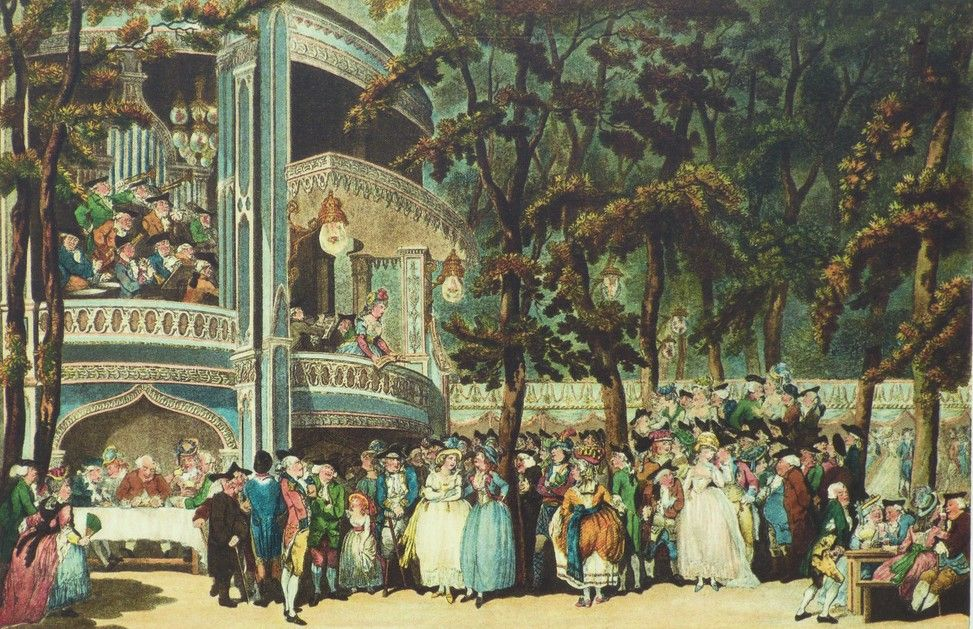
\includegraphics[width=0.7\textwidth]{vauxhall}
  \caption{Vauxhall Gardens \cite{900years}}
  \label{fig:Slika_Vauxhall}
\end{figure}

Svjetski sajmovi utjecali su na razvijanje koncepta trajnog parka namijenenog zabavi. Prvi svjetski sajam počeo je 1851. godine konstrukcijom Kristalne palače u Londonu u Engleskoj. Njegova svrha je bila proslava industrijskog napretka, te je dizajniran za edukaciju i zabavu posjetitelja. Posjetilo ga je 6 miliona ljudi, te je po ugledu na njega organiziran niz svjetskih sajmova širom Europe, a kasnije i Amerike. Svjetska kolumbijska izložba, organizirana 1893. godine u Chicagu u Sjedinjenim Američkim Državama se smatra pretečom modernih zabavnih parkova, s obzirom na brojne sadržaje koje su kasnije svi zabavni parkovi imali, poput vožnji, igara, svjetala, iluzija, te prvog željeznog vrtuljka\cite{worldfairs}. Uskoro su postala popularna različita odmarališta uz rijeke, jezera ili mora, koja su nudila različite zabavne sadržaje za svoje posjetitelje. U njima je izgrađen i prvi voz smrti (eng.\textit{rollercoaster}), izgrađen u Pennsylvaniji u Sjedinjenim Američkim Državama, te najstariji vrtuljak (karusel), izgrađen 1780. godine za princa Wilhelma IX od Hessen-Kassela, te, iako nije funkcionalan, može se vidjeti u Wilhelmsbad Parku u Hanauu u Njemačkoj, rodnom gradu braće Grimm \cite{900years}. 

\begin{figure}[h!]
  \centering
  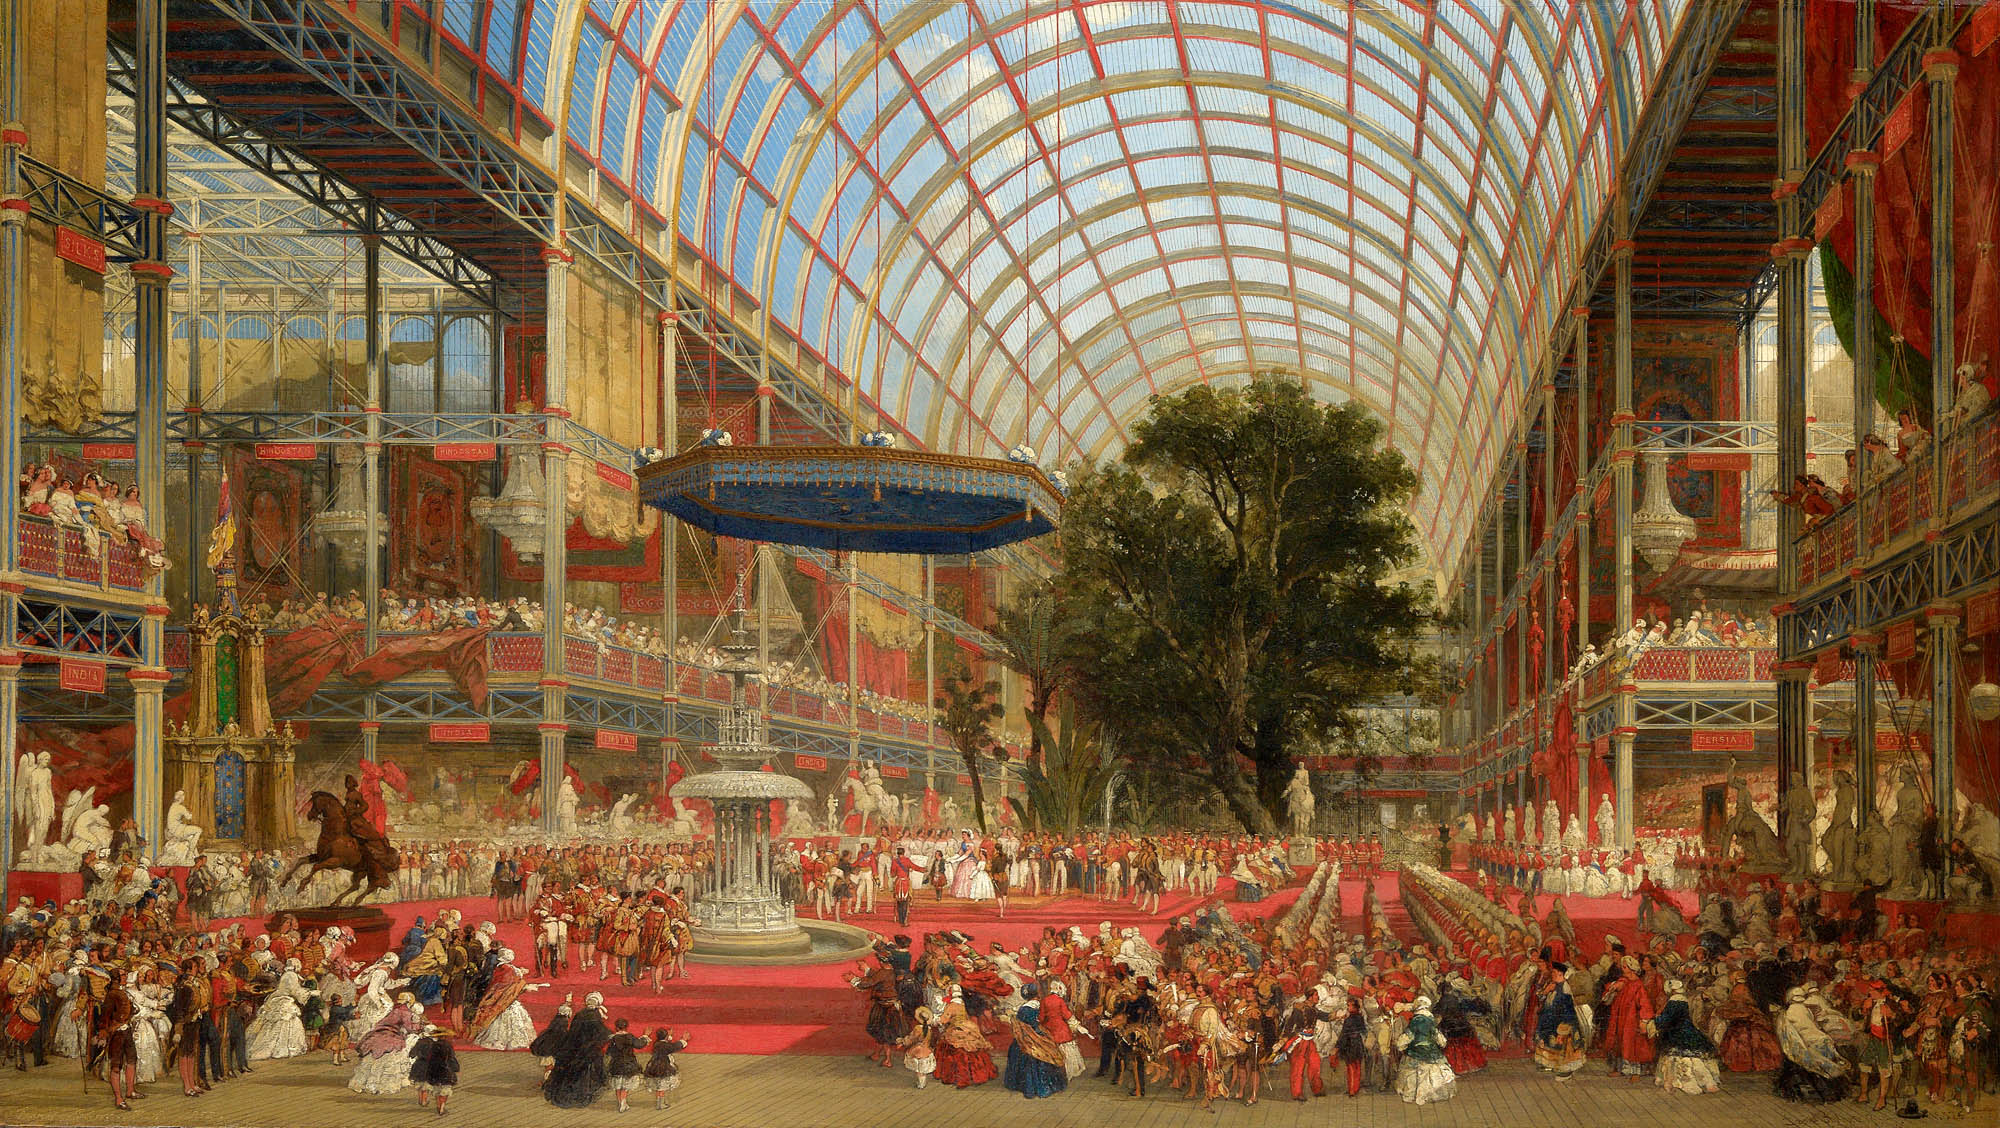
\includegraphics[width=0.7\textwidth]{fair}
  \caption{Prvi svjetski sajam, ulje na platnu od Davida Robertsa \cite{rct}}
  \label{fig:Slika_sajaml}
\end{figure}

Početkom 20. stoljeća, željezničke kompanije su, kako bi ostvarivale profit i vikendom, kad se ljudi manje kreću pošto ne putuju na posao i natrag, počeli otvarati takozvane \textit{trolley} parkove, koji su u početku imali dešavanja poput plesova, koncerata, vatrometa, a kasnije dobili gotovo sve sadržaje koje imaju današnji zabavni parkovi, poput vrtuljaka, vrteški, vozova smrti, i slično, te raznih restorana, vožnji brodovima, bazena, te brojnih drugih zabavnih sadržaja. Smatraju se pretečama današnjih zabavnih parkova. Jedan od najpopularnijih i najuspješnijih bio je Coney Island, pokraj autoputa u Coney Islandu u Brooklynu. Procjenjuje se da je u ovom periodu u Sjedinjenim Američkim Državama bilo između 1500 i 2000 \textit{trolley} parkova. Njihova popularnost se smanjila kad se povećala popularnost automobila \cite{kolica}.

\begin{figure}[h!]
  \centering
  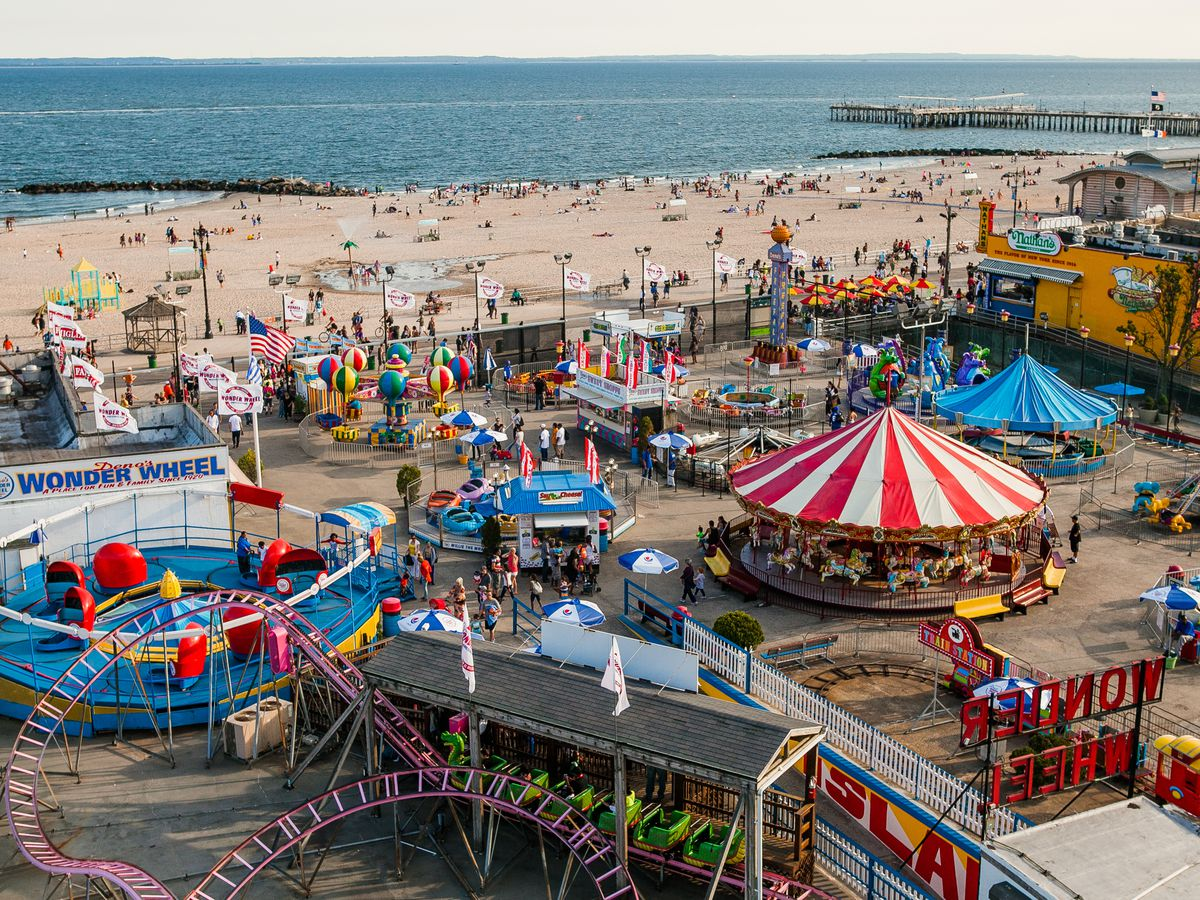
\includegraphics[width=0.7\textwidth]{coney}
  \caption{Coney Island u New Yorku \cite{coney}}
  \label{fig:Slika_Coney}
\end{figure}

Prvo trajno zatvoreno područje namijenjeno zabavi kojim upravlja jedna kompanija osnovano je 1895. godine u Coney Islandu u Brooklynu, a zvalo se Sea Lion Park. To je bio prvi zabavni park u kojem se, osim ulaza, plaćao i pristup pojedinim atrakcijama. Kad mu se 1897. godine pridružio Steeplechase Park, zbog blizine centra sa jako velikim brojem stanovništva, te lakoće pristupa, Coney Island je postao utjelovljenje američkog zabavnog parka. Njegovi dijelovi su bili i Luna Park, te Dreamland \cite{american}. Zbog velike popularnosti, uskoro su diljem svijeta otvoreni brojni zabavni parkovi pod imenom lunapark, a samo ime je ušlo u bosanski jezik kao sinonim za zabavni park. 

Period od 1920. godine do Velike depresije 1930. godine, te Drugog svjetskog rata se smatra zlatnim dobom zabavnih parkova. Radno vrijeme u Sjedinjenim Američkim Državama se skratilo, a plate povećale, pa su ljudi imali više slobodnog vremena i novca. U ovom periodu je najviše zabavnih parkova otvoreno, te je izmišljeno najviše atrakcija za njih \cite{american}. U pedesetim godinama se promijenio način kako ljudi provode slobodno vrijeme, populacija se zbog rata preselila izvan gradova, te je porasla popularnost televizije kao izvora zabave, a popularnost zabavnih parkova se jako smanjila. Tad su brojni zabavni parkovi zatvoreni ili zapaljeni. Walt Disney je napravio veliki rizik otvorivši veliki zabavni park pod svojim imenom, odnosno jedan od prvih tematskih parkova na svijetu, te mu se isti i isplatio, pošto je postao uzor za sve kasnije otvorene tematske parkove, te je svaki otvoreni Disneyev tematski park i danas na listi od 20 najposjećenijih tematskih parkova na svijetu \cite{900years}\cite{tematski}. 

Velike međunarodne kompanije, kao što su već spomenuta Walt Disney Company, te Universal Studios, Six Flags Entertainment Corporation, te Merlin Entertainments, vlasnik Legolanda, do 2020. godine su samo u Aziji uložile 24 milijarde dolara za izdradnju 60 tematskih parkova. Planira se gradnja ruskog odgovora Disneylandu, Magical World of Rusia, koji će vrijediti 4 milijarde dolara. Prvotno planiran za 2020. godinu, a zbog pandemije Covid-19 odgođen na oktobar 2021. godine, 2020 World Expo (Svjetski sajam 2020. godine) bit će organiziran u Dubaiju, te će sadržavati brojne zabavne i tematske parkove \cite{900years}. 

Zabavni parkovi, osim zabave, ostvaruju veliku ekonomsku dobit, dovode ogroman broj turista, te zapošljavaju veliki broj ljudi, bilo na projektovanju atrakcija ili na njihovom održavanju.


%Poglavlje 2
\chapter{Dizajn i implementacija}

Proces dizajniranja i implementacije, odnosno, projektovanja sistema, može se posmatrati kao proces rješavanja problema. Sam proces zahtijeva da se prvo pronađe niz mogućih rješenja, a zatim od pronađenih izabere najbolje rješenje. Svaki sistem mora biti projektovan na vrijeme, u okviru sredstava, imati prihvatljive performanse, te biti ispravan i pouzdan. Dobro projektovan sistem ne treba samo zadovoljiti trenutne zahtjeve, već i imati mogućnost da se prilagodi novim zahtjevima. 

Neki veliki lunapark obično projektuje tim ljudi. Određen broj ljudi zadužen je za planiranje arhitekture lunaparka, drugi tim ljudi zadužen je za planiranje tehničkog dijela, a posebni timovi zaduženi su za sam proces gradnje, a često sistem ima i tim zadužen za marketing. S obzirom da je ovo studentski projekt, simulacija lunaparka, sav posao, umjesto timova, radi jedan student. Sistem je sastavljen od podsistema, koje čine određene komponente uklopljene u objekte, najčešće napravljene od kartona. Sve to povezuje Arduino Mega mikrokontroler, programiran kôdom predstavljenim u nastavku seminarskog rada. 

 
\section{Maketa sistema}
Sistem se sastoji od jako detaljne makete, te elektronskih komponenti koje mu daju funkcionalnost. Dijelovi sistema su karusel, vrtuljak, šoljice, vračara, te igra koja uključuje sortiranje boja. Svi dijelovi su raspoređeni u ručno napravljene šatore ili na postolja. 
 \begin{figure}[h!]
  \centering
  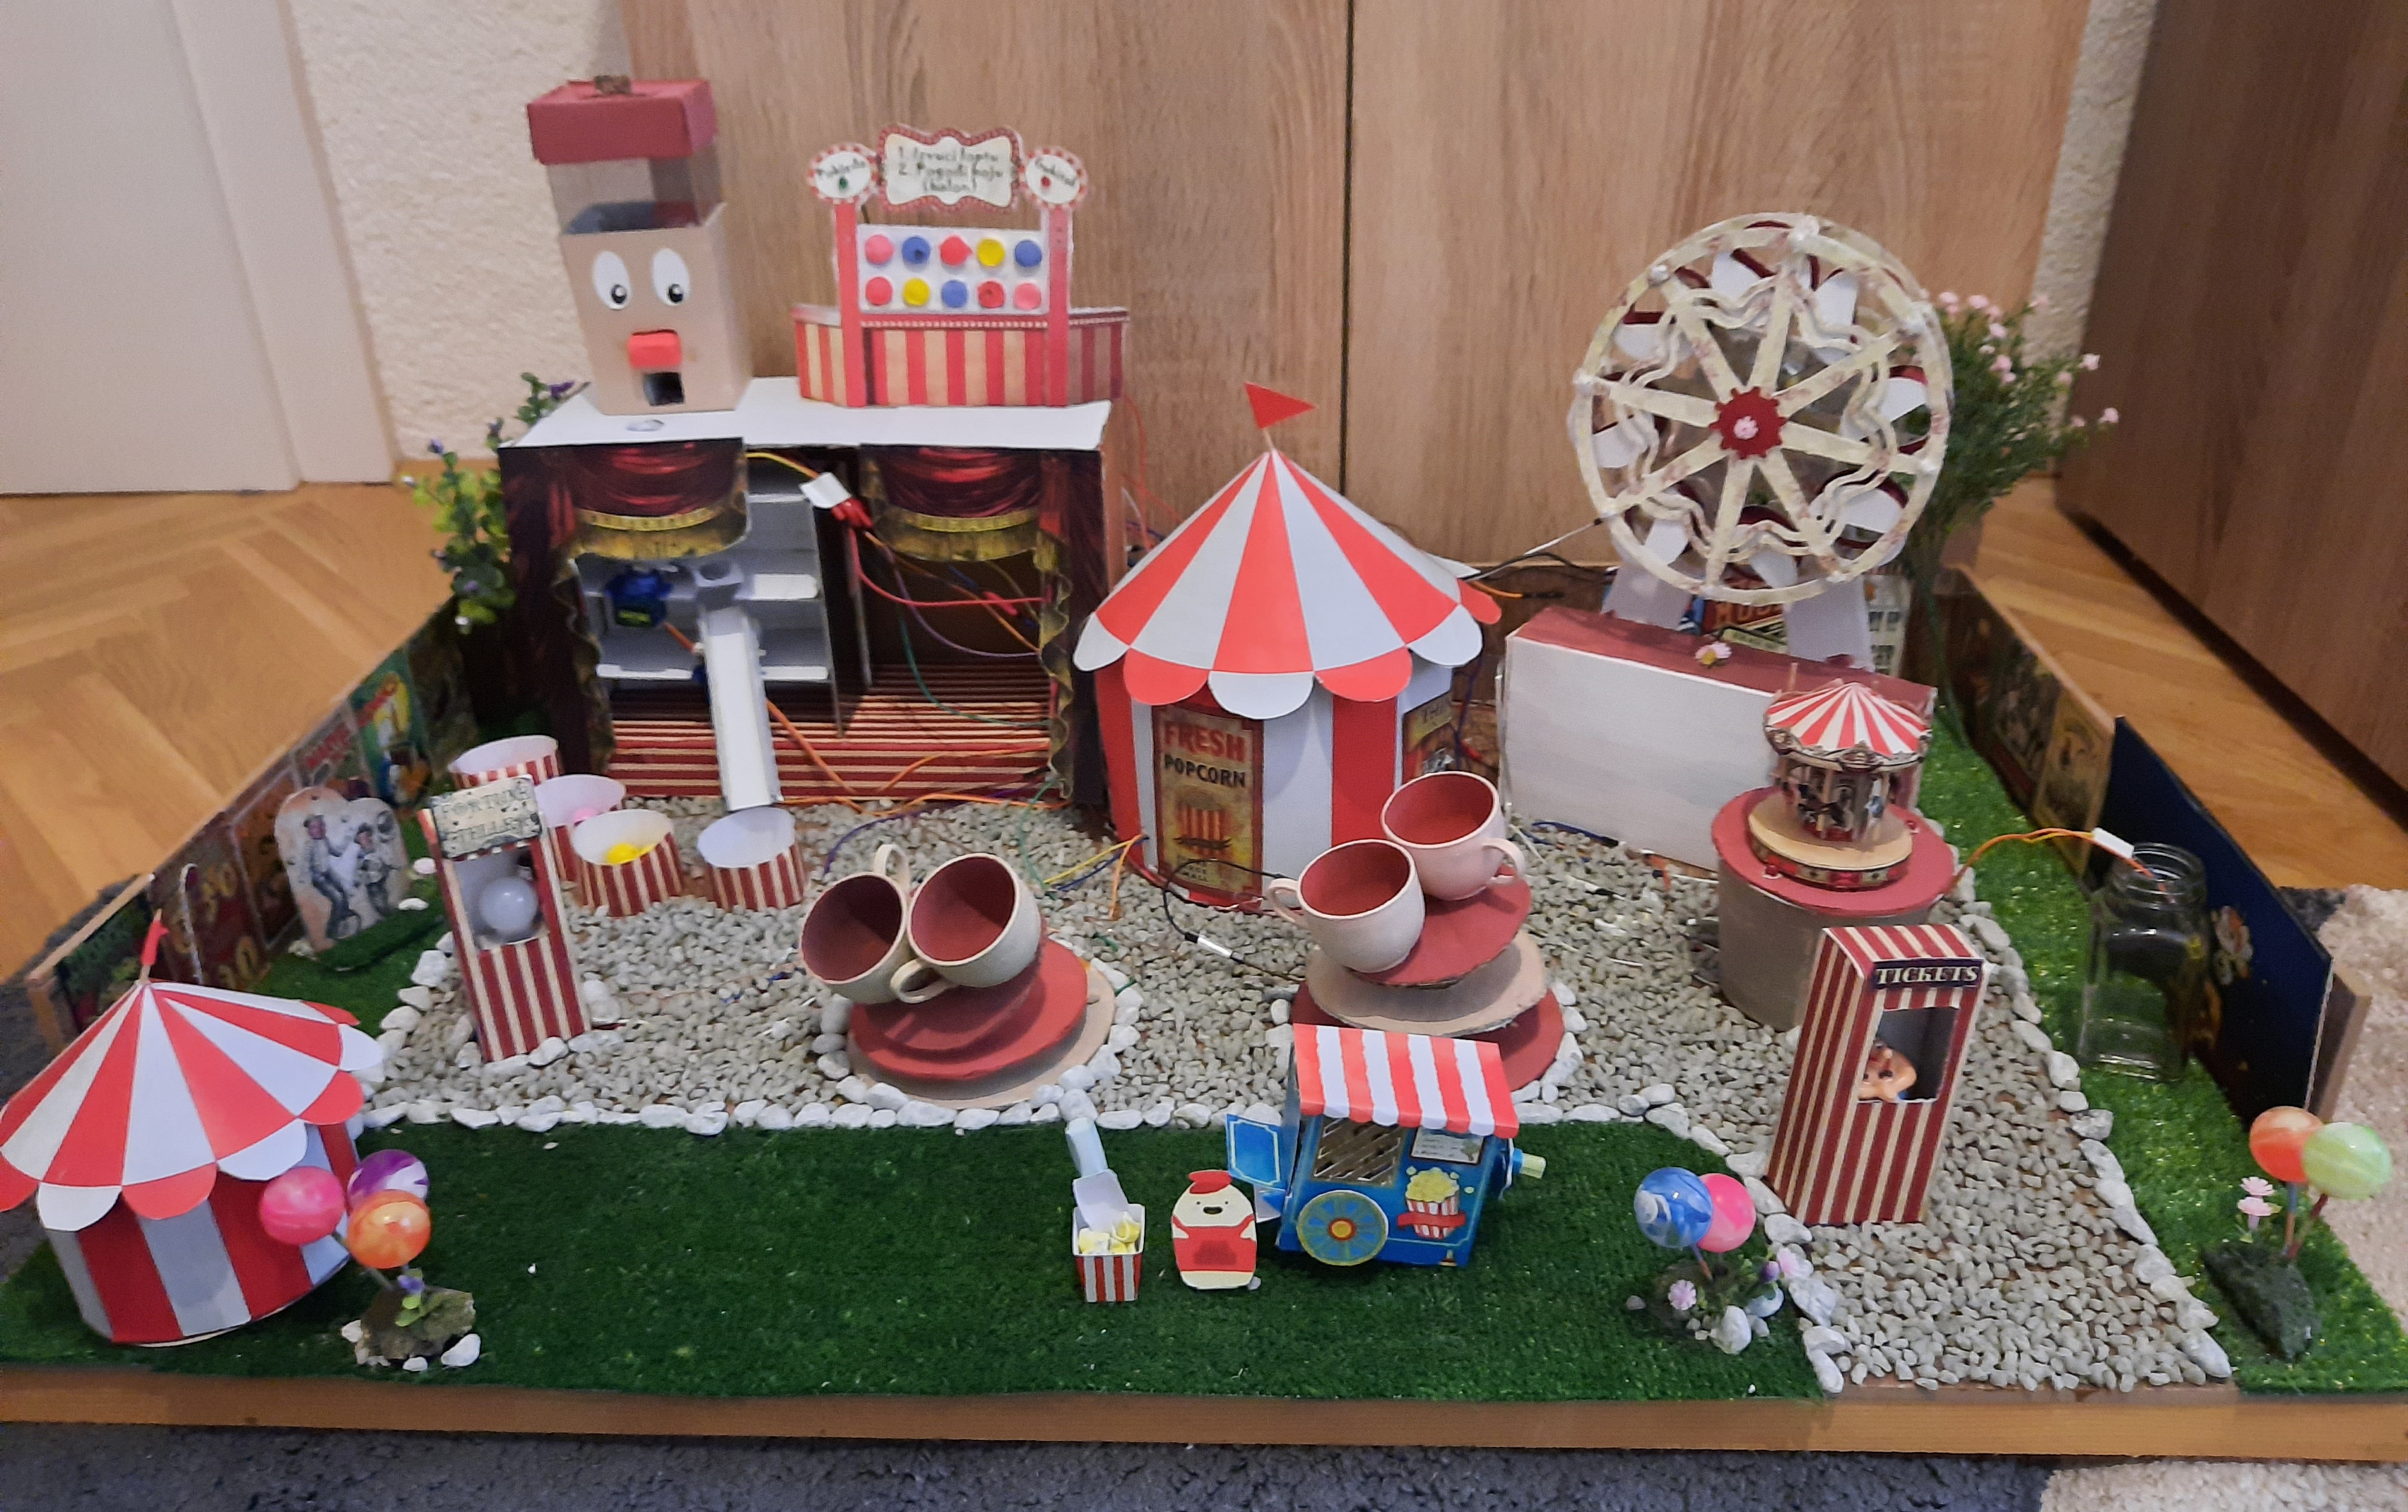
\includegraphics[width=0.7\textwidth]{maketa3}
  \caption{Maketa sistema}
  \label{fig:Slika_Maketa}
\end{figure}

Maketa sistema prikazana je na slici \ref{fig:Slika_Maketa}. Podloga je napravljena od šperploče, s tim da su zidovi, radi sigurnosti i stabilnosti, učvršćeni letvicama. Za nju nije korišteno ljepilo, već je pričvršćena ekserima. Posteri na zidovima su isprintani. Većina dijelova je napravljena od kartona, na koji su zalijepljeni šabloni od papira, koji su ili napravljeni u Photoshopu, ili preuzeti s Interneta, ali prilagođeni projektu. 

Shema sistema prikazana je na slici \ref{fig:Slika_shema}.
\begin{figure}[h!]
  \centering
  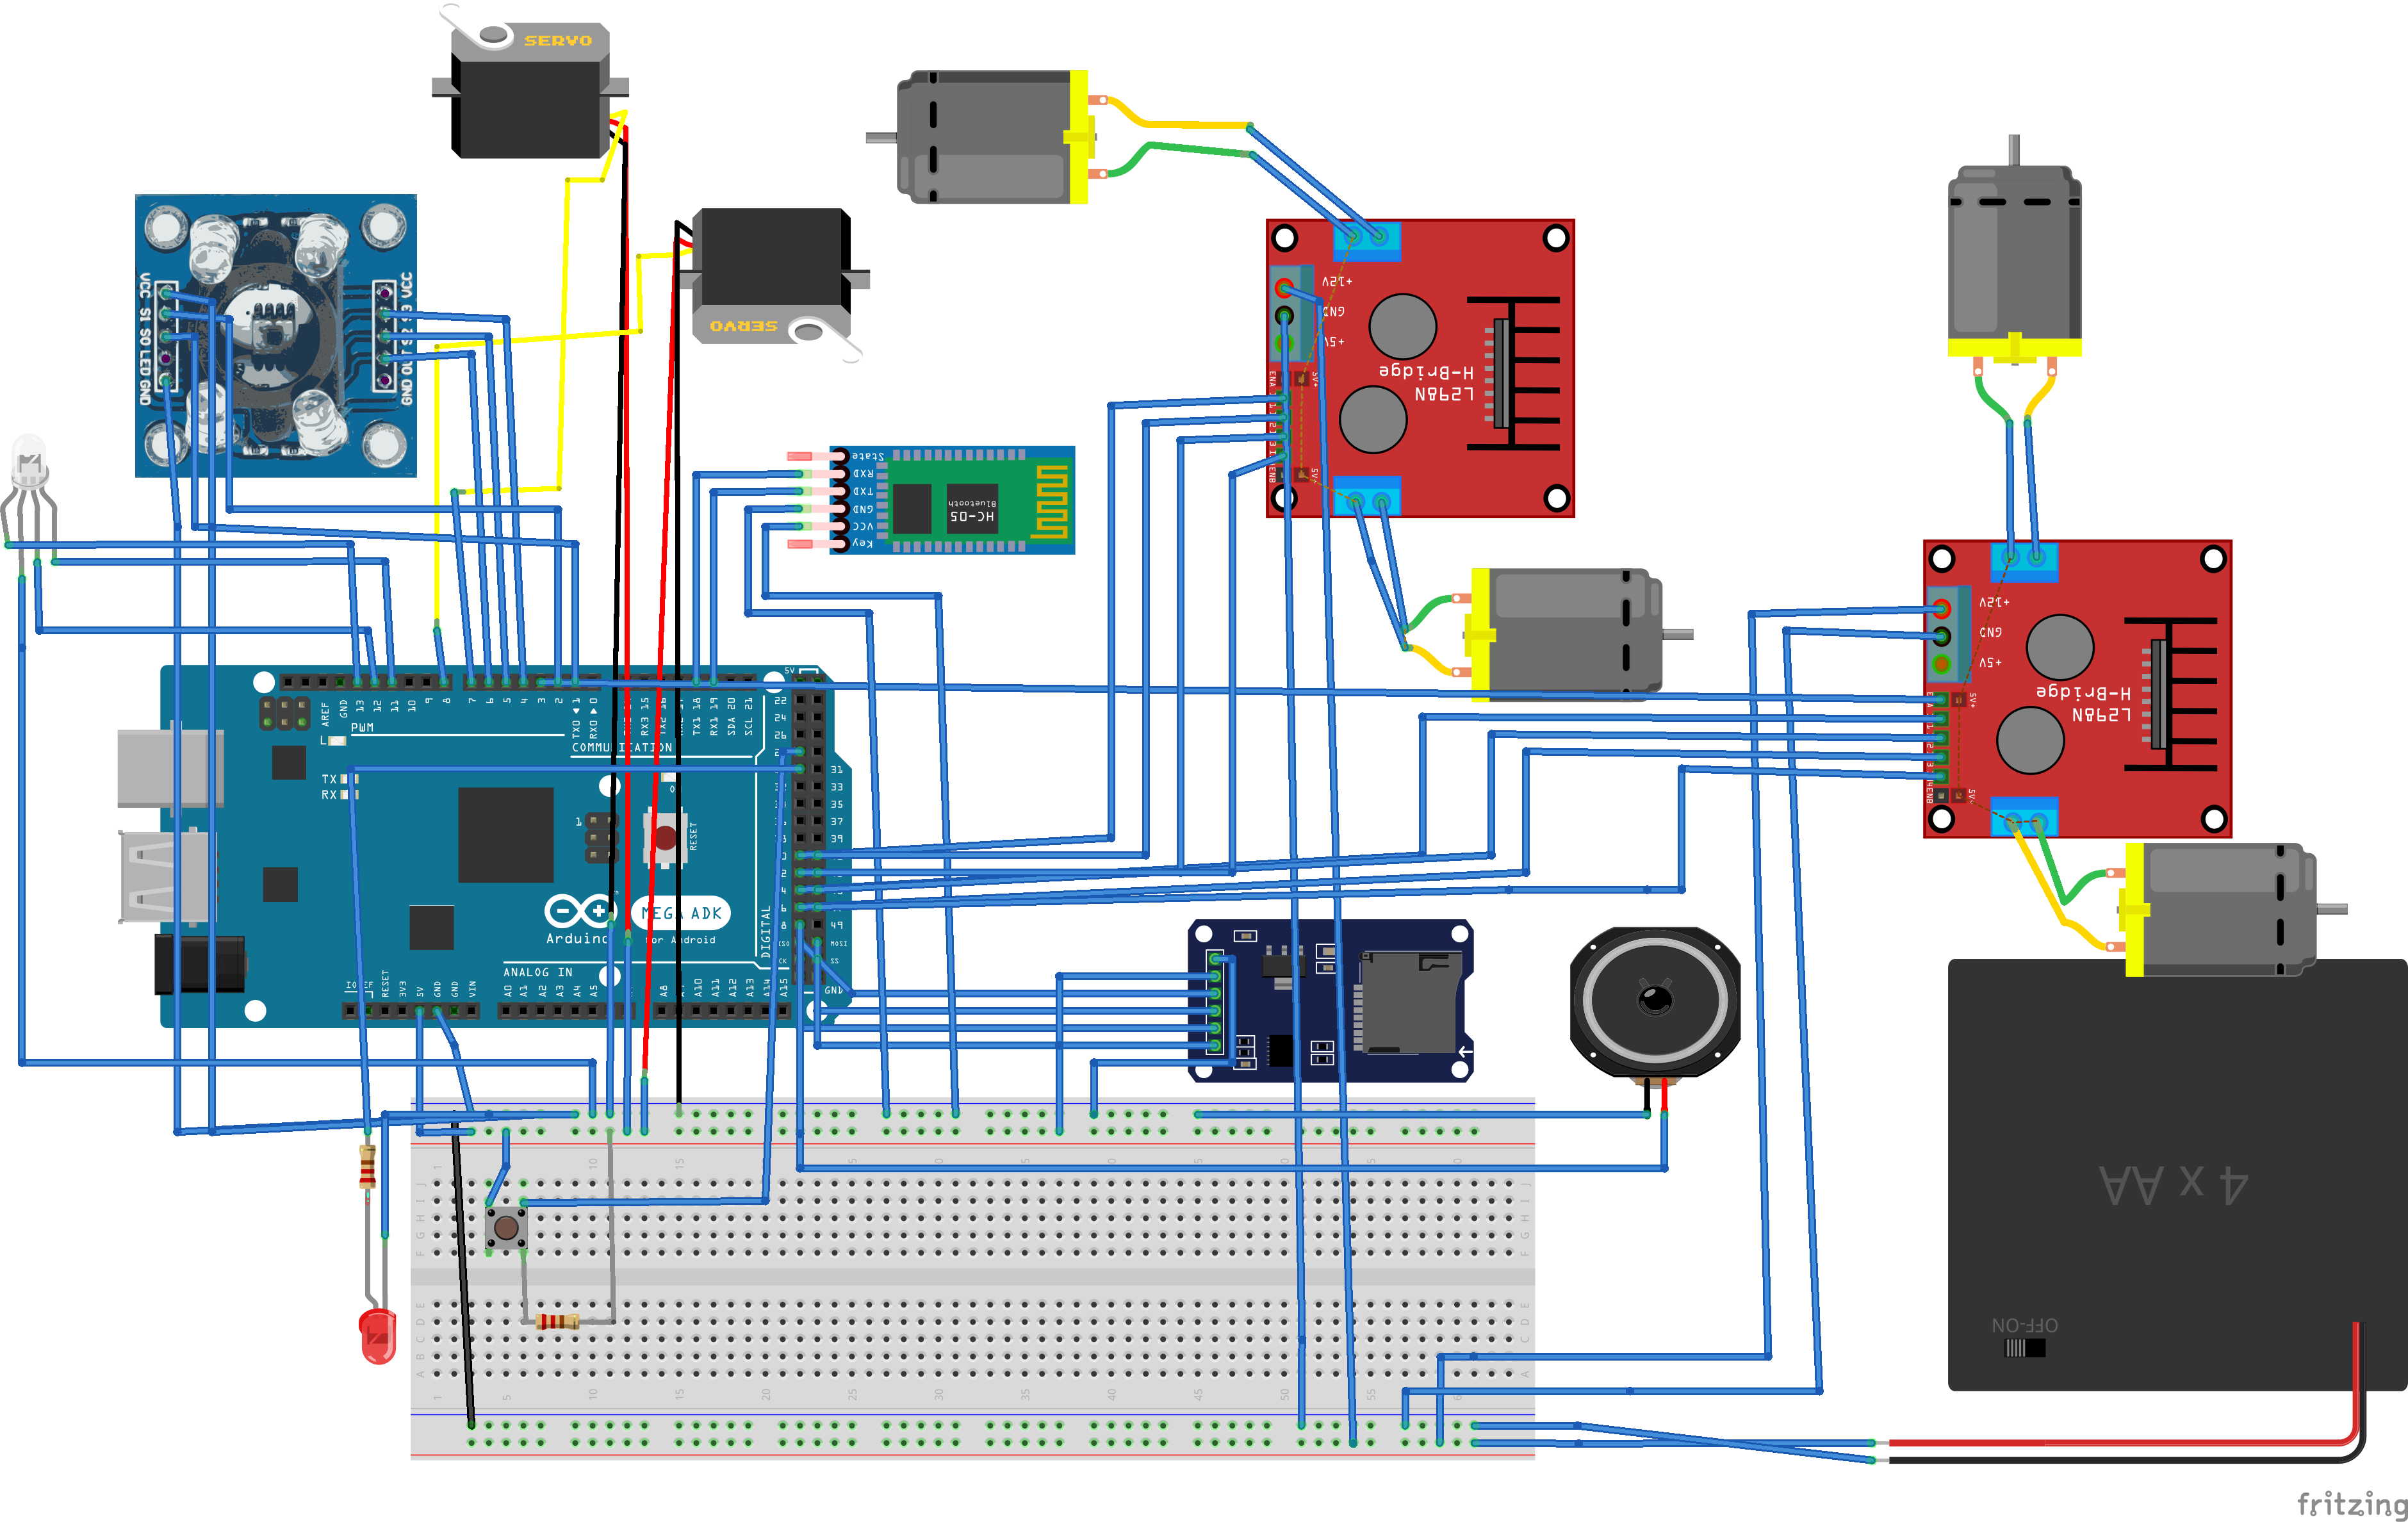
\includegraphics[width=0.7\textwidth]{shema2}
  \caption{Shema sistema}
  \label{fig:Slika_shema}
\end{figure}

Shema je malo pojednostavljena, duple diode i push buttoni nisu stavljeni. Električna shema prikazana je na slici \ref{fig:Slika_elshema}. 

\begin{figure}[h!]
  \centering
  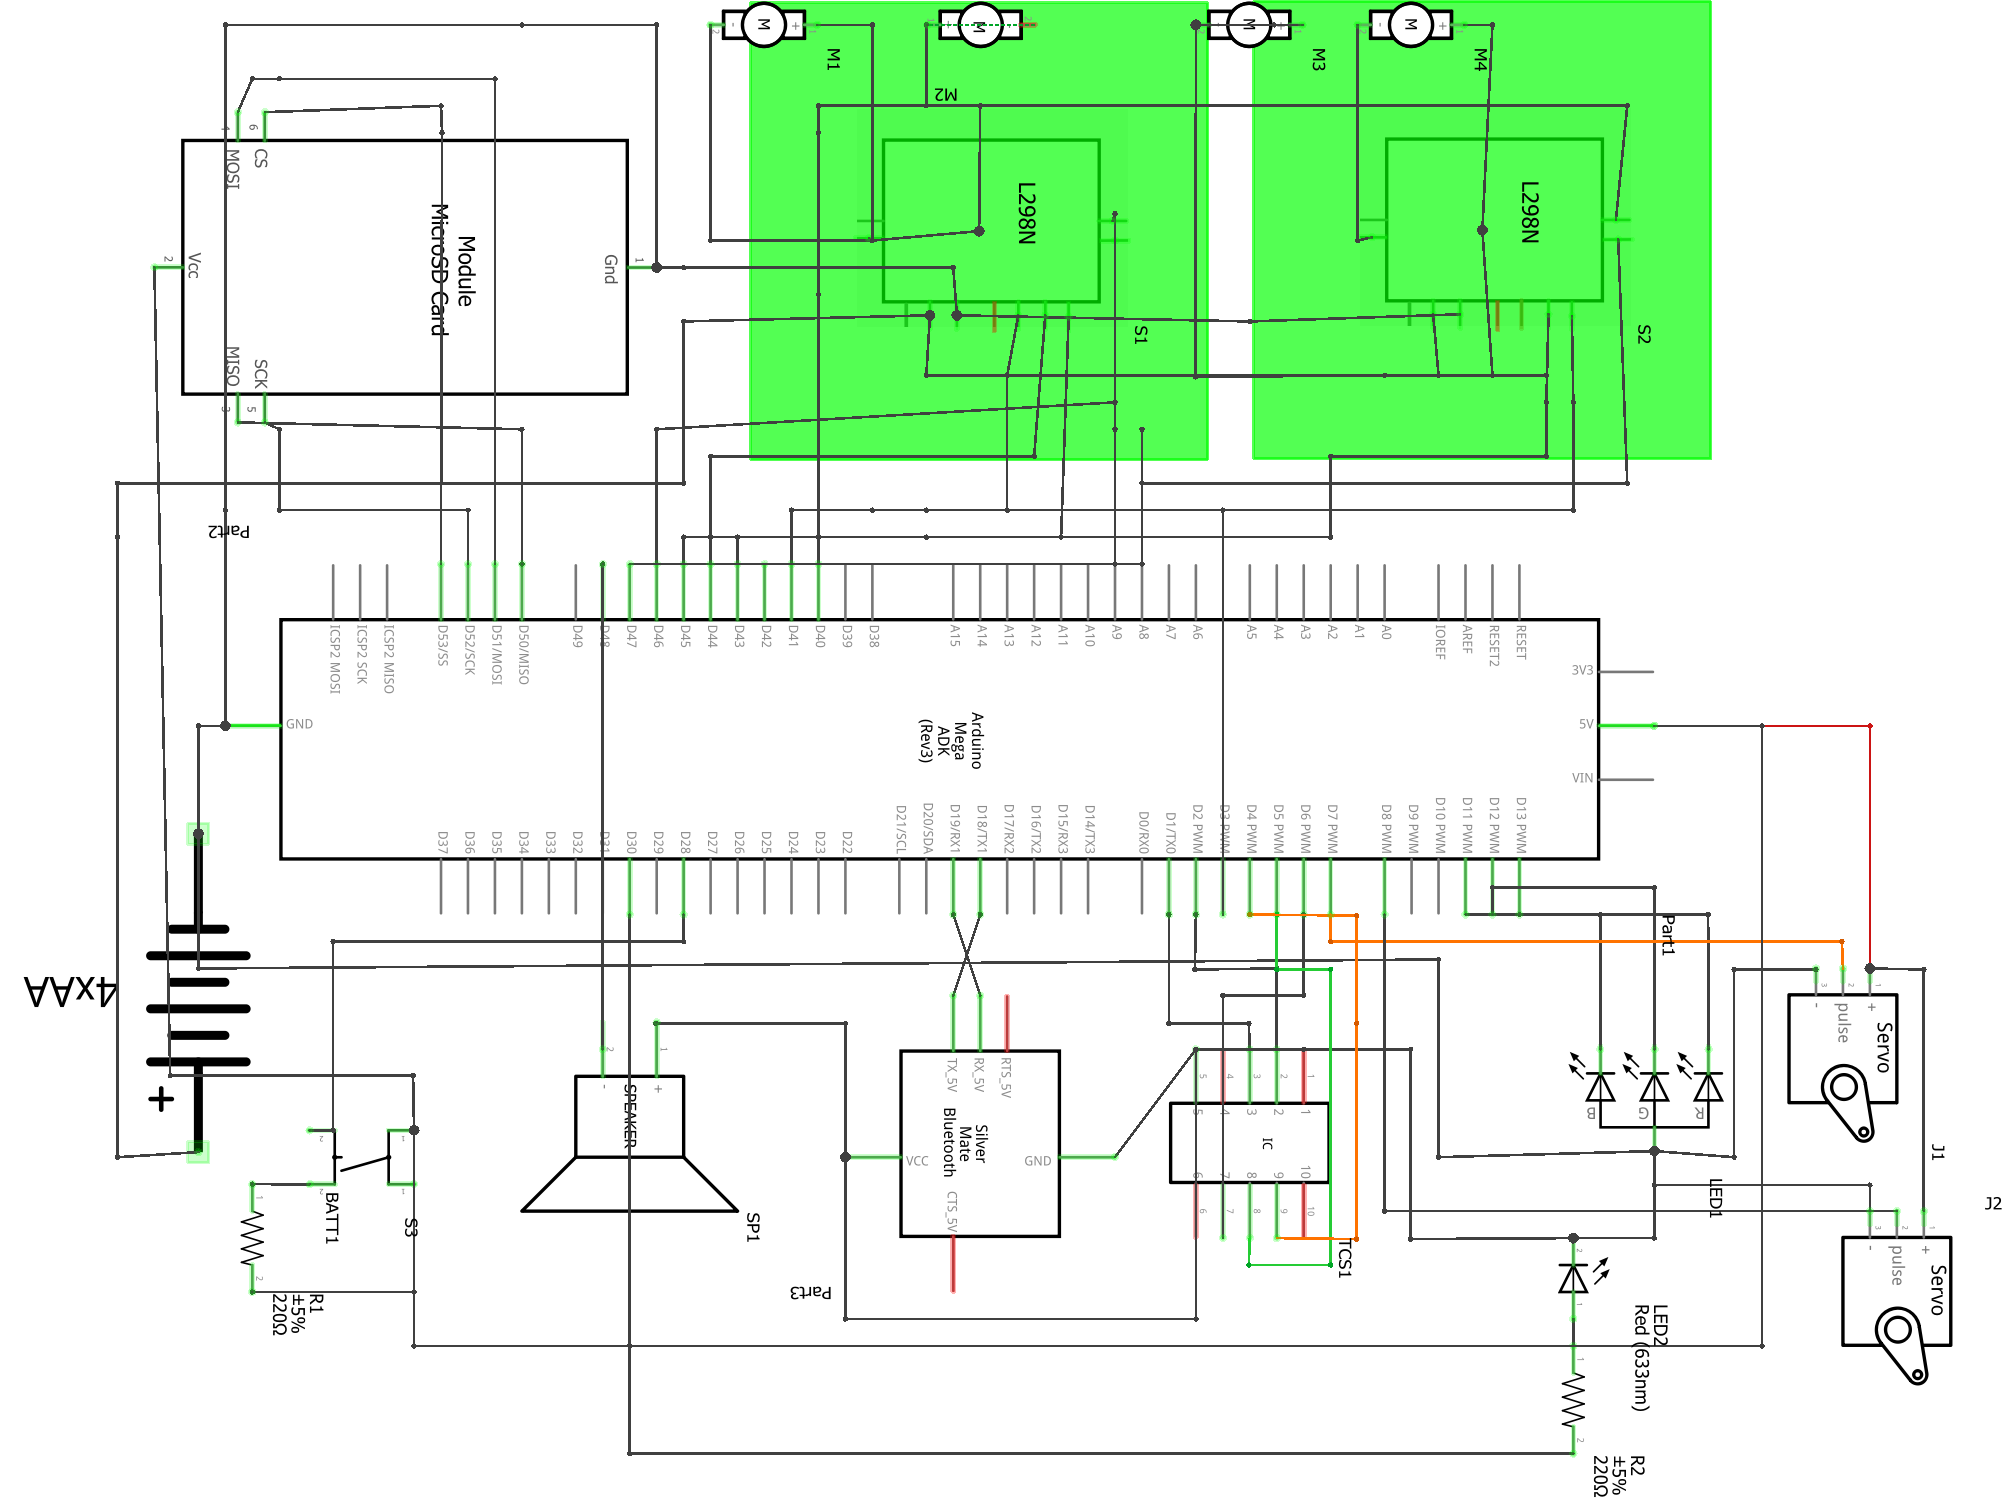
\includegraphics[width=0.7\textwidth]{elshema}
  \caption{Električna shema sistema}
  \label{fig:Slika_elshema}
\end{figure}

Na slici \ref{fig:Slika_dijagram} prikazan je blokovski dijagram sistema. Na dijagramu su označeni ulazi i izlazi iz sistema. Ulazi u sistem su napajanje, poruke primljene putem bluetootha, te informacije od senzora, modula i push buttona. Izlazi su signali koji se daju LED diodama, servo motorima, zvučniku, te motor driverima, koji ih prosljeđuju DC motorima. Motor driveri, osim signala od mikrokontrolera, primaju i vlastito napajanje, pošto nije dobro DC motore napajati zajedno s mikrokontrolerom. 

\begin{figure}[h!]
  \centering
  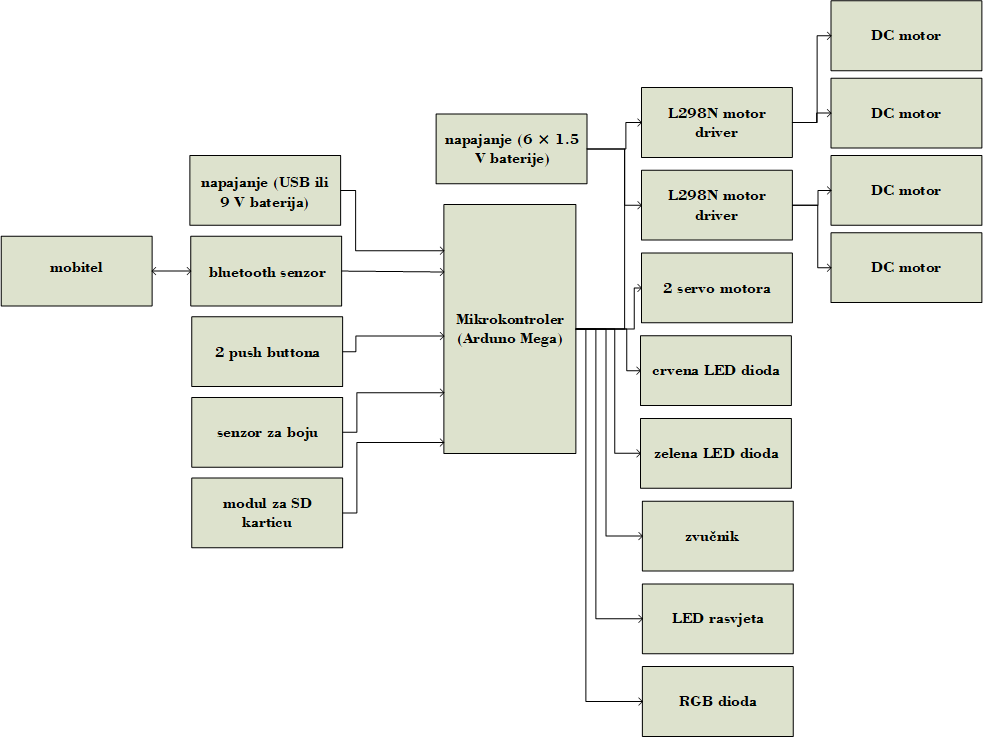
\includegraphics[width=0.7\textwidth]{dijagram}
  \caption{Blokovski dijagram sistema}
  \label{fig:Slika_dijagram}
\end{figure}

Osim komponenti, sistem se sastoji od Android aplikacije. Aplikacijom se simulira sistem za ulaznice u sistem. Korisnik pokaže ulaznicu radniku koji ima aplikaciju na mobitelu, te ako je ona odgovarajuća, korisnik može ući u sistem. Kad se pokrene Android aplikacija, otvori se prozor za prikazivanje ulaznice, kao na slici \ref{fig:Slika_prikazi}.

\begin{figure}[h!]
  \centering
  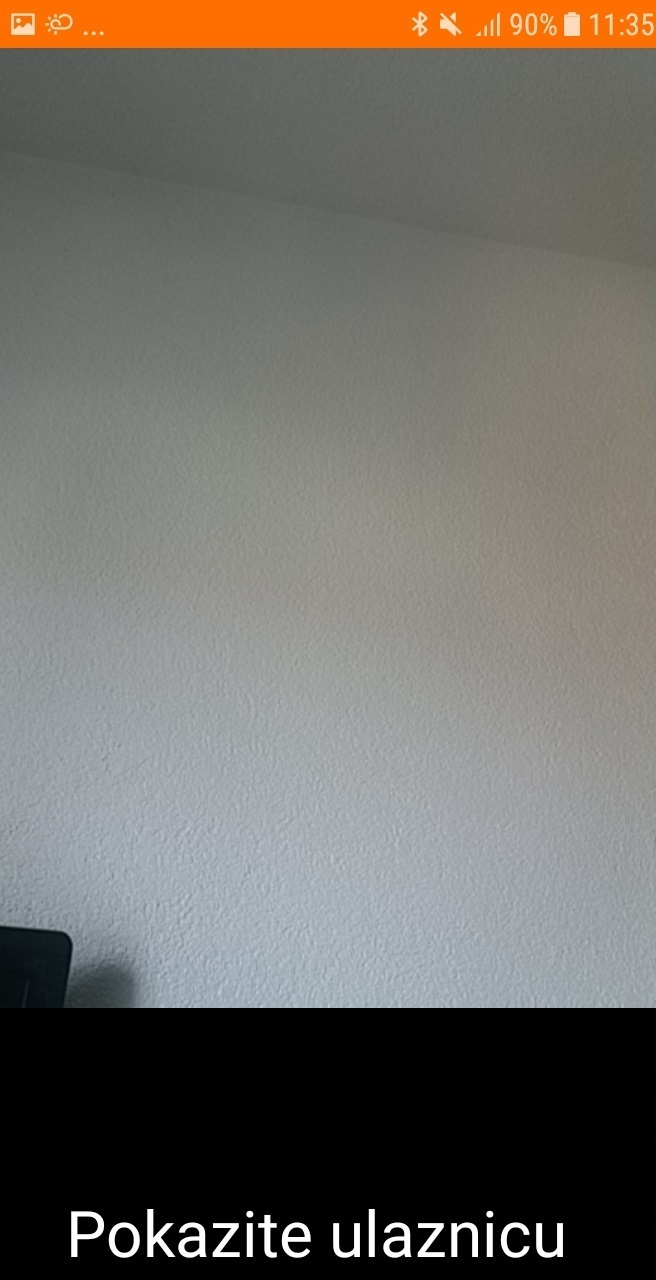
\includegraphics[width=0.25\textwidth]{prikazi}
  \caption{Izbornik za prikazivanje ulaznice}
  \label{fig:Slika_prikazi}
\end{figure}

Izrađene ulaznice prikazane su na slici \ref{fig:Slika_Ulaznice}. 
\newpage
\begin{figure}[h!]
  \centering
  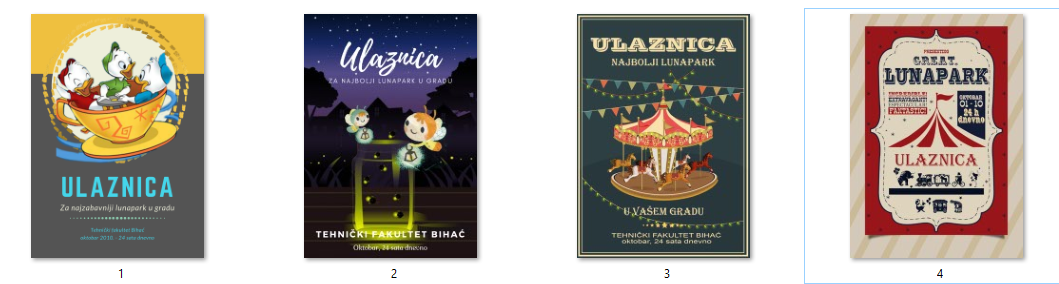
\includegraphics[width=0.7\textwidth]{ulaznice.png}
  \caption{Ulaznice za sistem}
  \label{fig:Slika_Ulaznice}
\end{figure}

Kad aplikacija prepozna ulaznicu, pokaže se izbornik za pretragu i povezivanje, kao na slici \ref{fig:Slika_izbornik}. Na istoj slici je prikazana i lista bluetooth uređaja koja se prikaže kad se pritisne izbornik za pretragu. Nakon povezivanja, otvori se izbornik kao na slici \ref{fig:Slika_kraj}. Uz pomoć ovog izbornika, korisnik upravlja sistemom.  
\begin{figure}[h!]
  \centering
  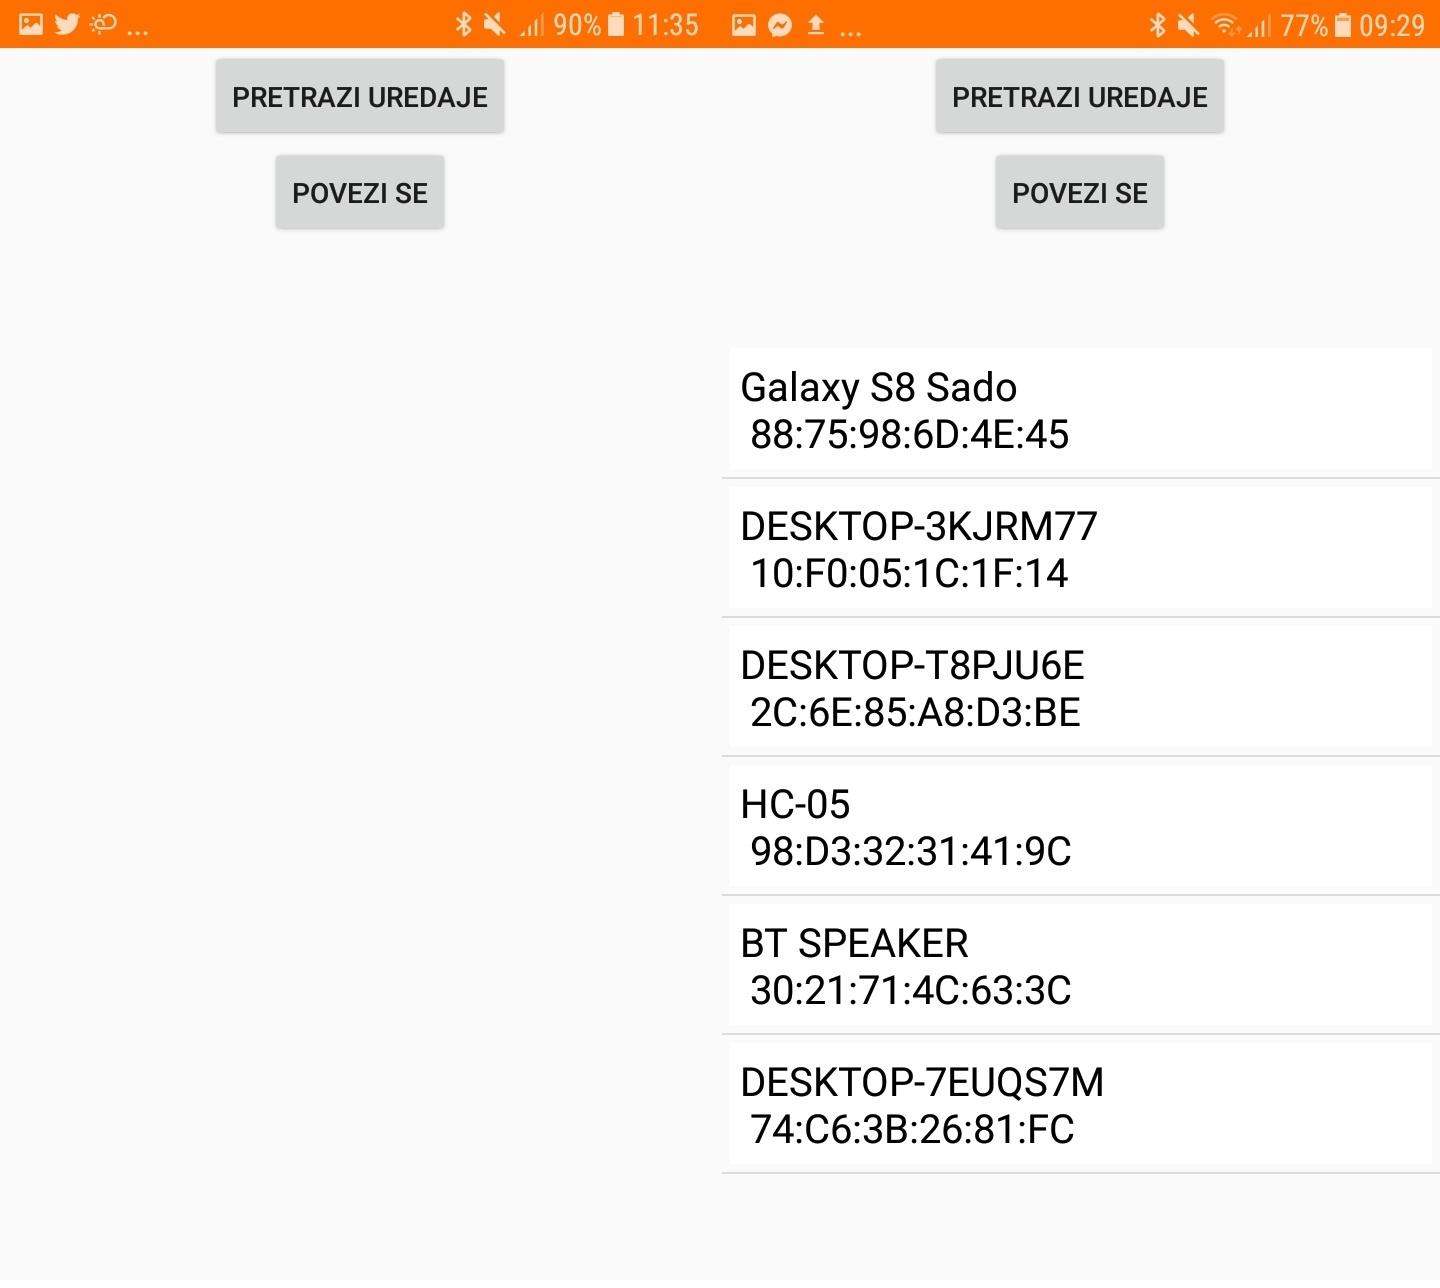
\includegraphics[width=0.5\textwidth]{pretrazibt}
  \caption{Izbornik za pretragu i povezivanje}
  \label{fig:Slika_izbornik}
\end{figure}

Blokovski dijagram podsistema za ulaznice prikazan je na slici \ref{fig:Slika_dijagram2}. Akvizicija ulaznice vrši se uz pomoć kamere mobitela. Prepoznavanje ulaznica vrši se uz pomoć neuronske mreže, koja šalje informaciju o prepoznavanju mobilnoj aplikaciji. Aplikacija potom komunicira sa sistemom uz pomoć bluetooth modula.

\begin{figure}[h!]
  \centering
  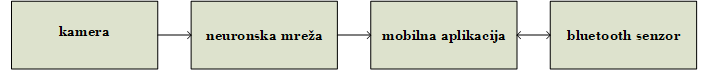
\includegraphics[width=0.7\textwidth]{dijagram2}
  \caption{Blokovski dijagram sistema za ulaznice}
  \label{fig:Slika_dijagram2}
\end{figure}

Komponente koje su iskorištene za kreiranje lunaparka su: Arduino Mega 2560 pločica, 4 različita DC motora (2 obična DC motora od 3 V, jedan od 12 V, a jedan sa zupčanicima), L298N driver za motore, modul za SD karticu, zvučnik, HC-05 Bluetooth modul, RGB dioda, senzor za boju, 2 servo motora, 3 push buttona, eskperimentalna pločica, te diode i otpornici.

\begin{figure}[h!]
  \centering
  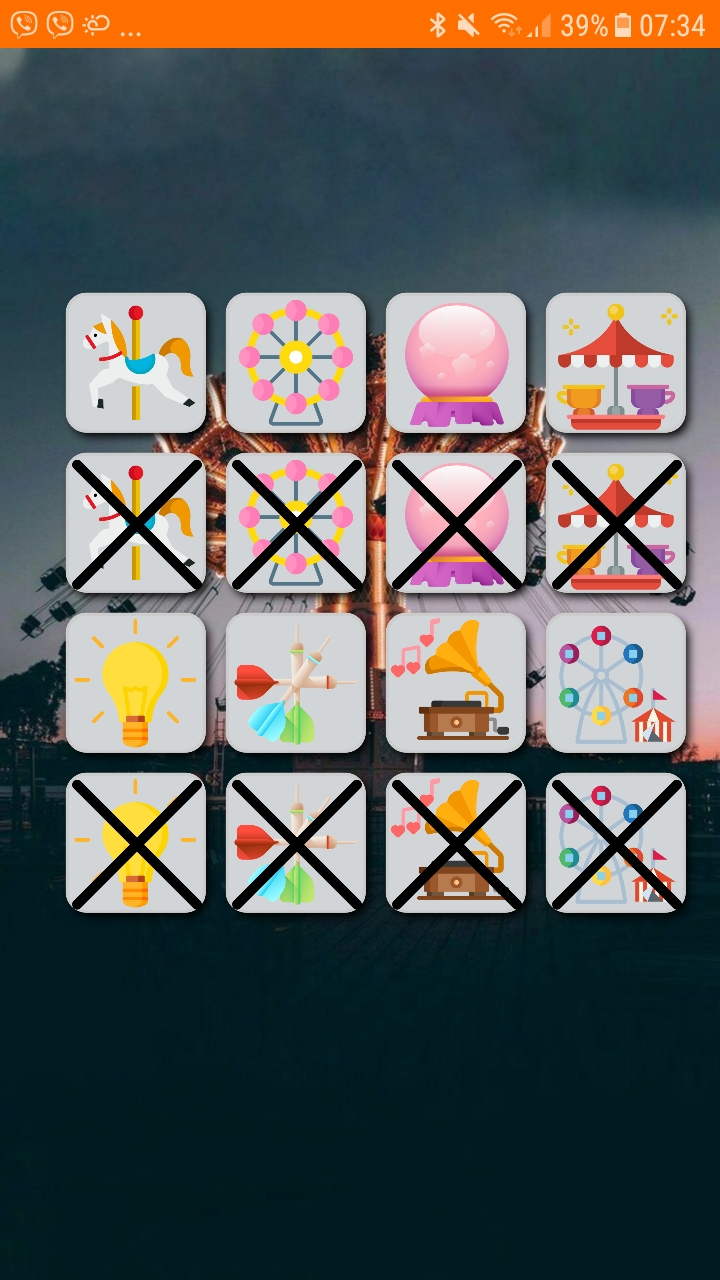
\includegraphics[width=0.25\textwidth]{kraj2}
  \caption{Finalni izbornik aplikacije}
  \label{fig:Slika_kraj}
\end{figure}

Većina komponenti smještena je u veliki šator na sredini makete, kako ne bi kvarile sam dizajn projekta. Unutrašnjost šatora prikazana je na slici \ref{fig:Slika_sator}. Posebna pažnja morala je da se obrati na to da komponente budu povezane s odgovarajućim pinovima. Bluetooth modul morao je biti povezan sa serijskim portom, kojih Arduino Mega ima čak 4, modul za SD karticu morao je biti povezan sa posljednja 4 pina, pošto su to MISO (\textit{Master In Slave Out}), MOSI (\textit{Master Out Slave In}), SCK (\textit{Serial Clock}) i SS (\textit{Slave Select}) pinovi, pinovi namijenjeni za asihnhronu komunikaciju u kojoj je Arduino pločica master element, dok su RGB dioda i kontrola brzine motora morali biti povezani sa PWM pinovima.
\begin{figure}[h!]
  \centering
  \includegraphics[width=0.5\textwidth]{unutrasnjost}
  \caption{Unutrašnjost šatora u kojem je skrivena većina komponenti}
  \label{fig:Slika_sator}
\end{figure}

Motorima u sistemu obezbijeđeno je vlastito napajanje, pomoću paketa od 6 AA baterija od 1,5 V, dok se Arduino pločica i ostale komponente mogu napajati uz pomoć USB-a, odnosno, električne energije, ili baterije od 9 V. Na ovaj način sistem je osiguran od pregaranja, a istovremeno je omogućeno dovoljno energije da se veliki broj motora kreće kako je planirano.
\
%Poglavlje 3
\chapter{Programiranje sistema}

\section{Arduino kôd}
Arduino programski jezik temelji se na Wiring programskom okviru za upravljanje mikrokontrolerima, a Arduino softver temelji se na Processing softveru. Wiring je sličan C++ programskom jeziku, ali je djelomično pojednostavljen i izmijenjen. Wiring i Processing su, kao i Arduino, \textit{open source}, odnosno otvorenog kôda, dostupni besplatno, zajedno sa svim projektima i doprinosima korisnika.

Cijeli programski kôd ovog sistema dan je prilogu. On se sastoji od uvođenja svih biblioteka potrebnih za rad, deklarisanja varijabli, funkcija za rad pojedinih dijelova, te \textit{setup()} i \textit{loop()} funkcija. U \textit{setup()} funkciji su sve radnje koje se pokreću čim se mikrokontroler pokrene, a u \textit{loop()} funkciji radnje koje se ponavljaju beskonačno mnogo puta dok god mikrokontroler ima ulazni napon.  

Ono što se u ovom sistemu beskonačno mnogo puta ponavlja je čitanje podataka koji se primaju preko Bluetootha. 
Loop se neprestano vrti dok god je pločica priključena na napon. Tu se čitaju primljeni podaci s bluetooth senzora, i prema njima pokreću funkcije. Ako je korisnik pritisnuo button za pokretanje vrteške, ona se počne vrtiti, ako je pritisnuo za zaustavljanje, ona stane, i tako dalje.
 \begin{lstlisting}[frame=single,language=C++,numbers=left, numberstyle=\tiny, xleftmargin=0.05\textwidth, xrightmargin=0.05\textwidth, basicstyle=\ttfamily\footnotesize]
 void loop(){
 
while(Serial1.available()==0) ;

if(Serial1.available()>0) {
data = Serial1.parseInt();
 
} 

delay(400);

\end{lstlisting}

U varijablu \textit{data} spremaju se brojevi primljeni preko bluetooth senzora. Njihova vrijednost je definisana u aplikaciji napravljenoj pomoću Android studija. U toj aplikaciji, na primjer, ako korisnik pritisne button za uključenje dioda, preko Bluetootha se šalje broj 67, a ako pritisne button za gašenje dioda, preko bluetootha se šalje broj 76. Shodno tome, aplikacija mikrokontrolera, ako primi broj 67, treba uključiti diode, a ako primi broj 76, treba ih isključiti.
 \begin{lstlisting}[frame=single,language=C++,numbers=left, numberstyle=\tiny, xleftmargin=0.05\textwidth, xrightmargin=0.05\textwidth, basicstyle=\ttfamily\footnotesize]
 if (data == 67){
  diodeUkljuci();
}
if (data == 76){
  diodeIskljuci();
}

\end{lstlisting}

Na analogan način je napravljena veza između aplikacije i svih drugih dijelova sistema, samo, naravno, sa različitim vrijednostima koje se šalju preko bluetootha.
 \begin{lstlisting}[frame=single,language=C++,numbers=left, numberstyle=\tiny, xleftmargin=0.05\textwidth, xrightmargin=0.05\textwidth, basicstyle=\ttfamily\footnotesize]
if (data == 23){
  vracara();
}
if (data == 32){
  vracaraUgasi();
}
\end{lstlisting}

Vračara ima svoju kristalnu kuglu, čije se boje mijenjaju promjenom boja RGB diode.
   \begin{lstlisting}[frame=single,language=C++,numbers=left, numberstyle=\tiny, xleftmargin=0.05\textwidth, xrightmargin=0.05\textwidth, basicstyle=\ttfamily\footnotesize] 
void vracara(){
  RGB_color(255, 0, 0); // crvena
  delay(1000);
  RGB_color(0, 255, 0); // zelena
  delay(1000);
  RGB_color(0, 0, 255); // plava
  delay(1000);
  RGB_color(255, 255, 125); // roza
  delay(1000);
  RGB_color(0, 255, 255); // cijan
  delay(1000);
  RGB_color(255, 0, 255); // magenta
  delay(1000);
  RGB_color(255, 255, 0); // zuta
  delay(1000);
  RGB_color(255, 255, 255); // bijela
  delay(1000);
}


void RGB_color(int crvena, int zelena, int plava) {
  analogWrite(crveni_pin, crvena);
  analogWrite(zeleni_pin, zelena);
  analogWrite(plavi_pin, plava);
}
 \end{lstlisting}
 
Senzor za boje osvijetli lopticu uz pomoć jedne od tri diode, prvo crvene (R), pa zelene (G), pa plave (B), a onda čita vrijednost dobijene frekvencije da dobije zastupljenost boje koju ta dioda emitira na loptici.

 \begin{lstlisting}[frame=single,language=C++,numbers=left, numberstyle=\tiny, xleftmargin=0.05\textwidth, xrightmargin=0.05\textwidth, basicstyle=\ttfamily\footnotesize]
int readColor() {
// Citanje crvenih fotodioda
  digitalWrite(S2, LOW);
  digitalWrite(S3, LOW);
  frekvencija = pulseIn(sensorOut, LOW);
  int R = frekvencija;
    delay(50);

// Citanje zelenih fotodioda
  digitalWrite(S2, HIGH);
  digitalWrite(S3, HIGH);
  frekvencija = pulseIn(sensorOut, LOW);
  int G = frekvencija;
  delay(50);
  
// Citanje plavih fotodioda
  digitalWrite(S2, LOW);
  digitalWrite(S3, HIGH);
  frekvencija = pulseIn(sensorOut, LOW);
  int B = frekvencja;
  delay(50);

  if((R<45 & R>32 & G<70 & G>50) || (R>70 & G<10 & B <50 & B>30) ){
    color = 1; // Crvena
  }
  if(R<45 & R>35 & B<40 &B>30){
    color = 2; // Roza
  }
  if(R<63 & R>50 & G<55 & G>45 & B<40 & B>29){
    color = 3; // Plava
  }
  if(R<40 & R>30 & G<50 & G>40 & B<46 & B>38){
    color = 4; // Zuta
  }
  return color;  
}
 \end{lstlisting}

Ako je pritisnut jedan od buttona, pokrese se dio programa. Ako korisnik pritisne odgovarajući button, te pogodi koje je boje loptica, on pobijedi, uključuje se zelena dioda, u suprotnom, uključuje se crvena. Loptica se uz pomoć servo motora i napravljenog mehanizma kreće, prvo do senzora za boju, gdje se očita njena boja, a onda u odgovarajuću posudu.

 \begin{lstlisting}[frame=single,language=C++,numbers=left, numberstyle=\tiny, xleftmargin=0.05\textwidth, xrightmargin=0.05\textwidth, basicstyle=\ttfamily\footnotesize]
void senzorZaBoje(){
   crveniButtonState = digitalRead(crveniButton);
   plaviButtonState = digitalRead(plaviButton);


  if (crveniButtonState == HIGH || plaviButtonState == HIGH) {
  gornjiServo.write(120);
  delay(3000);
  
  for(int i = 115; i > 55; i--) {
    gornjiServo.write(i);
    delay(2);
  }
  delay(1000);
  
  color = readColor();
  color = readColor();
  color = readColor();
  color = readColor();
  
  delay(1000);  
  switch (color) {
    case 1: //crvena
    if (crveniButtonState == HIGH){
      digitalWrite(zelenaDioda, HIGH);
      digitalWrite(crvenaDioda, LOW);
    }
    if (plaviButtonState == HIGH ){
      digitalWrite(crvenaDioda, HIGH);
      digitalWrite(zelenaDioda, LOW);
    }
    donjiServo.write(50);
    break;
    case 2: //roza
    digitalWrite(crvenaDioda, HIGH);
    digitalWrite(zelenaDioda, LOW);
    donjiServo.write(75);
    break;
    case 3: // zuta
      digitalWrite(crvenaDioda, HIGH);
      digitalWrite(zelenaDioda, LOW);
    donjiServo.write(100);
    break;
    case 4: // plava
     if (plaviButtonState == HIGH){
    digitalWrite(zelenaDioda, HIGH);
    digitalWrite(crvenaDioda, LOW);
    }
    if (crveniButtonState == HIGH ){
    digitalWrite(crvenaDioda, HIGH);
    digitalWrite(zelenaDioda, LOW);
    }
    donjiServo.write(125);
    break;  
    case 0:
    break;
  }
  delay(300);
  
  for(int i = 55; i > 20; i--) {
    gornjiServo.write(i);
    delay(2);
  } 
  delay(500);
  
  for(int i = 29; i < 115; i++) {
    gornjiServo.write(i);
    delay(2);
  }
  color=0;
  }
}
 \end{lstlisting}
 Motori se vrte stavljanjem pozitivnih i negativnih napona na njihove pinove.

 \begin{lstlisting}[frame=single,language=C++,numbers=left, numberstyle=\tiny, xleftmargin=0.05\textwidth, xrightmargin=0.05\textwidth, basicstyle=\ttfamily\footnotesize]
void vrtiMotore(){
  digitalWrite(motor1pin1, HIGH);
  digitalWrite(motor1pin2, LOW);

  digitalWrite(motor2pin1, HIGH);
  digitalWrite(motor2pin2, LOW);

  digitalWrite(motor3pin1, HIGH);
  digitalWrite(motor3pin2, LOW);
  
    analogWrite(enA, 160);  // upravljanje brzinom
  digitalWrite(motor4pin1, HIGH);
  digitalWrite(motor4pin2, LOW);
}
 \end{lstlisting}
 Na ovaj način isprogramiran je svaki dio sistema.

\section{Android Studio kôd}
Sve mobilne aplikacije napravljene uz pomoć softvera Android Studio sastoje se od takozvanih aktivnosti (eng. \textit{activities}). Jedna aktivnost predstavlja jednu radnju, koja najčešće zauzima cijeli ekran. Iz jedne aktivnosti u drugu prelazi se automatski, ili aktiviranjem nekog linka ili tipke na ekranu.

Prvi dio aplikacije napravljen je uz pomoć biblioteke od Tensorflowa za treniranje neuronske mreže, te prepoznavanje treniranih objekata u Android aplikaciji. Prepoznavanje slike je akcija kojom uređaj, koji izvrši akviziciju slike, u ovom slučaju preko kamere kao ulaza, prepozna koji je objekat na istoj, te ispiše kojoj klasi pripada. Moderni načini prepoznavanja slike su korištenjem dubokog učenja, odnosno, treniranjem konvolutivnih neuronskih mreža na ogromnim bazama podataka. Tensorflow, korišten za izradu programa, je \textit{open-source} platforma, odnosno platforma otvorenog kôda, za mašinsko učenje koja sadrži ogroman broj alata i biblioteka za olakšani razvoj aplikacija. Ovu platformu je razvio Google Brain, Googleov tim za umjetnu inteligenciju, prvotno samo za potrebe kompanije Google, a u novembru 2015. godine objavljen je za široku populaciju pod Apache 2.0 licencom. Može se koristiti za kreiranje algoritama za mašinsko učenje, te za pokretanje istih, a bez puno promjena može se pokrenuti na mnogim uređajima, od mobilnih telefona i tableta do velikih distribuiranih sistema sastavljenih od stotina ili hiljada uređaja poput GPU kartica \cite{Tensorflow}. 

Klasifikator za prepoznavanje slika u ovom projektu napravljen je treniranjem jednostavnog modela uz pomoć dubokog učenja sa online alatom kojeg je razvio Google, a koji se zove Teachable Machine. Treniranje modela prikazano je na slici \ref{fig:Slika_Treniranje}, a isti je eksportovan u TensorFlow lite datoteku, koja se može koristiti na Android uređajima.
\begin{figure}[h!]
  \centering
  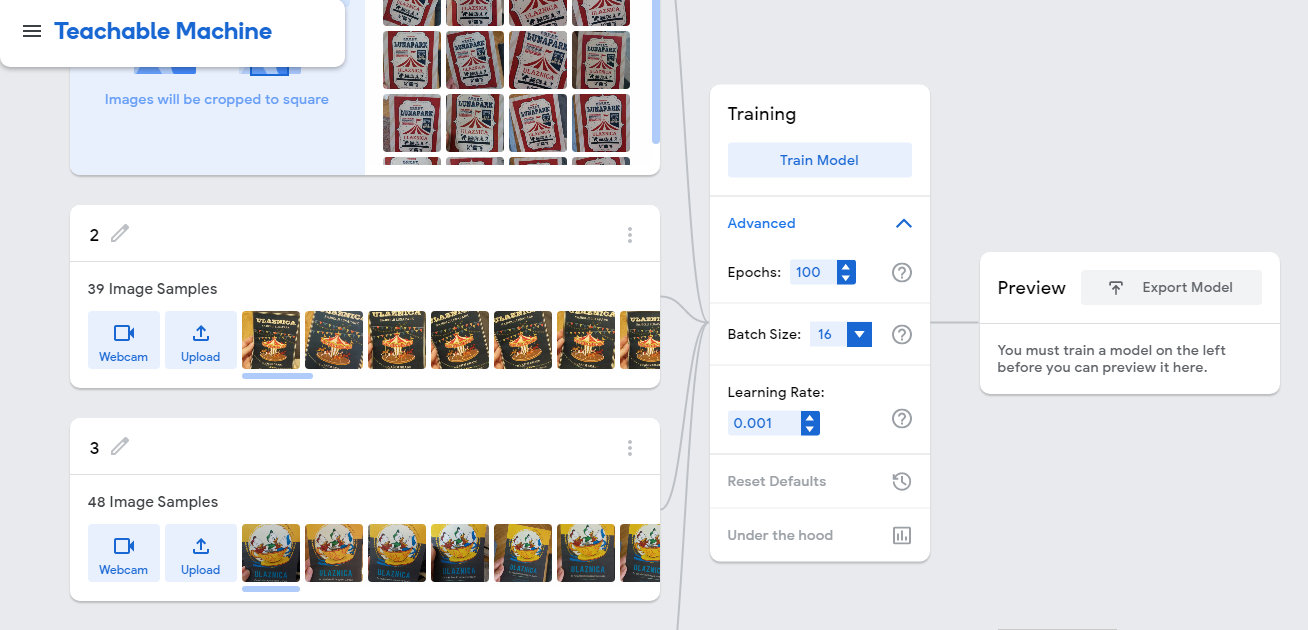
\includegraphics[width=0.8\textwidth]{treniranje.png}
  \caption{Treniranje neuronske mreže}
  \label{fig:Slika_Treniranje}
\end{figure}

Model se sastoji od slika ulaznica za lunapark, koje su kreirane u softveru Adobe Photoshop. Za projekat su napravljene 4 ulaznice, a njihove fotografije raspoređene su u 4 direktorija pomoću kojih je neuronska mreža istrenirana. TensorFlow nudi vlastitu aplikaciju otvorenog kôda za korištenje modela. Ista je izmijenjena da se prilagodi potrebama projekta.

Prvo što se korisniku prikaže je izlaz iz kamere njegovog mobitela, te poruka da pokaže ulaznicu. Bitan dio kôda je:

\begin{lstlisting}[frame=single,language=Java,numbers=left, numberstyle=\tiny, xleftmargin=0.05\textwidth, xrightmargin=0.05\textwidth, basicstyle=\ttfamily\footnotesize]
 protected void showResultsInBottomSheet(List<Recognition> results) {
    if (results != null && results.size() >= 3) {

      Recognition recognition = results.get(0);
      if (recognition != null) {

        if (recognition.getTitle() != null)
          recognitionTextView.setText(recognition.getTitle());
        System.out.println("name"+recognition.getTitle());

        System.out.println("namevalue"+recognition.getConfidence());
        if(recognition.getConfidence()<0.90f){
          result_text.setText("Pokazite ulaznicu"); 
          // ako je stepen prepoznavanja manji od 0.9, korisniku se ispisuje poruka da pokaze ulaznicu
        }
          if(recognition.getConfidence()>0.90f){
            result_text.setText(recognition.getTitle());
            Intent intent = new Intent(getApplicationContext(), BtActivity.class);
            startActivity(intent);
            // ako je stepen prepoznavanja veci od 0.9, korisnika se prebacuje na Bluetooth aktivnost
          }
          }
          \end{lstlisting}

Kad sistem prepozna ulaznicu, pokrene se sljedeća aktivnost, a to je izbornik za traženje dostupnih Bluetooth uređaja, te povezivanje na odgovarajući. Sastoji se od dva buttona, odnosno dugmeta, tipke, te liste Bluetooth uređaja koja nije vidljiva dok korisnik ne pokrene pretragu.

Kad korisnik dodirne dugme za pretragu, ispiše mu se lista dostupnih bluetooth uređaja:

\begin{lstlisting}[frame=single,language=Java,numbers=left, numberstyle=\tiny, xleftmargin=0.05\textwidth, xrightmargin=0.05\textwidth, basicstyle=\ttfamily\footnotesize]
pretraga.setOnClickListener(new View.OnClickListener() {

            @Override
            public void onClick(View arg0) {
                mBTAdapter = BluetoothAdapter.getDefaultAdapter(); // povezivanje na bluetooth adapter

                if (mBTAdapter == null) {
                    Toast.makeText(getApplicationContext(), "Bluetooth uredajii nisu pronadeni", Toast.LENGTH_SHORT).show(); // poruka ako nije pronaden ni jedan uredaj
                } else if (!mBTAdapter.isEnabled()) {
                    Intent enableBT = new Intent(BluetoothAdapter.ACTION_REQUEST_ENABLE);
                    startActivityForResult(enableBT, BT_ENABLE_REQUEST);
                } else {
                    new SearchDevices().execute(); // pretraga uredeja
                }
            }
        });
        \end{lstlisting}
 Ako korisnik nije povezan na bluetooth, otvori se poruka da ga je potrebno uključiti. Pretraga uređaja vrši se sljedećim dijelom kôda:
        \begin{lstlisting}[frame=single,language=Java,numbers=left, numberstyle=\tiny, xleftmargin=0.05\textwidth, xrightmargin=0.05\textwidth, basicstyle=\ttfamily\footnotesize]
   private class SearchDevices extends AsyncTask<Void, Void, List<BluetoothDevice>> {

        @Override
        protected List<BluetoothDevice> doInBackground(Void... params) {
            Set<BluetoothDevice> pairedDevices = mBTAdapter.getBondedDevices();
            List<BluetoothDevice> listDevices = new ArrayList<BluetoothDevice>(); // kreiranje liste
            for (BluetoothDevice device : pairedDevices) {
                listDevices.add(device); // stavljanje uredaja u listu
            }
            return listDevices;

        }
\end{lstlisting}

Kad korisnik klikne na dugme za povezivanje, pokrene se povezivanje na odabrani bluetooth uređaj:

\begin{lstlisting}[frame=single,language=Java,numbers=left, numberstyle=\tiny, xleftmargin=0.05\textwidth, xrightmargin=0.05\textwidth, basicstyle=\ttfamily\footnotesize]
connect.setOnClickListener(new View.OnClickListener() {

            @Override
            public void onClick(View arg0) {
                BluetoothDevice device = ((MyAdapter) (listView.getAdapter())).getSelectedItem();
                Intent intent = new Intent(getApplicationContext(), ControllingActivity.class); // novi intent 
                intent.putExtra(DEVICE_EXTRA, device); // stavljanje podataka o uredaju u intent
                intent.putExtra(DEVICE_UUID, mDeviceUUID.toString());
                intent.putExtra(BUFFER_SIZE, mBufferSize);
                startActivity(intent); // zapocinjanje aktivnosti
            }
        });
\end{lstlisting}

Također se izvršio prijelaz u sljedeću aktivnost, kreiranjem takozvanog intenta, pomoću kojeg se započinje aktivnost \textit{ControllingActivity}, koja je zadužena za samo upravljanje lunaparkom. U toj aplikaciji nalazi se izbornik za pokretanje i zaustavljanje sistema, te pokretanje i zaustavljanje muzike, sastavljen od buttona. 

\begin{lstlisting}[frame=single,language=Java,numbers=left, numberstyle=\tiny, xleftmargin=0.05\textwidth, xrightmargin=0.05\textwidth, basicstyle=\ttfamily\footnotesize]
connect.setOnClickListener(new View.OnClickListener() {
btnMuzika.setOnClickListener(new View.OnClickListener()
        {

            @Override
            public void onClick(View v) {

                try {
                    mBTSocket.getOutputStream().write(pokreni.getBytes());

                } catch (IOException e) {
                    // TODO Auto-generated catch block
                    e.printStackTrace();
                }
            }});
            \end{lstlisting}
            
Osim funkcionalnosti, svaki dio je potrebno definisati u XML datoteci zaduženoj za dizajn same aplikacije, odnosno, pozicioniranje njenih dijelova i stavljanje određene slike kao pozadine.
\begin{lstlisting}[frame=single,language=XML,numbers=left, numberstyle=\tiny, xleftmargin=0.05\textwidth, xrightmargin=0.05\textwidth, basicstyle=\ttfamily\footnotesize]
connect.setOnClickListener(new View.OnClickListener() {
<Button
        android:id="@+id/muzika"
        android:layout_width="150dp"
        android:layout_height="100dp"
        android:text="Muzika"
        android:layout_marginTop="420dp"
        android:layout_marginLeft="20dp"
        android:background="@drawable/muzika"
        />
   \end{lstlisting}         
Kôd za svaki button je sličan, pa nema potrebe da se svaki stavi u rad. Kad se dodirne button, preko bluetootha se šalje određen niz bajtova povezanom uređaju. Arduinov bluetooth modul prima te nizove bajtova, a u kôdu aplikacije specifirano je koja se radnja izvrši nakon primanja kojeg niza bajtova.

\section{Komunikacija mikrokontrolera i vanjskih uređaja}

Mikrokontroler koristi različite načine komunikacije s vanjskim uređajima. U sklopu ovog sistema, vršeno je direktno čitanje izlaznih signala, serijska i master-slave komunikacija.

\begin{figure}[h!]
  \centering
  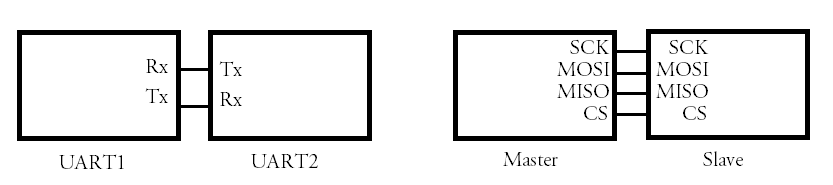
\includegraphics[width=0.8\textwidth]{komunikacija}
  \caption{Serijska i master-slave komunikacija}
  \label{fig:Slika_Komunikacija}
\end{figure}

Kod čitanja stanja push buttona, te kontrole LED dioda, te motora, komunikacija je ostvarena direktnim čitanjem stanja elemenata sistema. Stanje može biti niski napon, odnosno logička nula, ili visoki napon, logička jedinica. Naprimjer, ako je push button pritisnut, on na povezani pin šalje logičku jedinicu, te prema tome sistem započinje kretanje servo motora i očitavanje boje. 

Komunikacija sa mobilnim uređajem ostvarena je uz pomoć bluetooth modula koji je povezan serijski s mikrokontrolerom preko UART modula, kao na lijevoj strani slike \ref{fig:Slika_Komunikacija}. UART modul pretvara paralelni prikazane podatke sa registara u serijski prikazane podatke, odnosno niz bizova. HC-05 modul omogućuje full duplex komunikaciju, odnosno, oba učesnika u komunikaciji mogu biti i prijemnici, i predajnici, te su linije za prijenos i primanje podataka odvojene. Ovaj modul također omogućuje i sinhronu, i asinhronu komunikaciju - i u odgovarajućim, i u nasumičnim intervalima. 

Komunikacija sa modulom za SD karticu ostvarena je preko SPI interfejsa, kao na desnoj strani slike \ref{fig:Slika_Komunikacija}, koji je sinhronog tipa. Kod ovog interfejsa, jedan uređaj je master, odnosno, onaj koji inicira početak prijenosa komunikacije. U ovom slučaju to je mikrokontroler. Modul za SD karticu je slave, te se s njega preko linija za prijenos podataka isti prenose, onda kada master mikrokontroler preko upravljačkih linija to inicira.
%Poglavlje 4
\chapter{Eksperimentalna analiza rada sistema}

Krerani sistem napravljen je od nekoliko podsistema koji su usklađeni u jednu cjelinu.

Prvi podsistem je osvjetljenje, rpikazano na slici \ref{fig:Slika_osvjetljenje}, postignuto pojedinačnim LED diodama, te LED svjetlima iz novogodišnjeg ukrasa. Uključuje se i isključuje po korisnikovoj želji uz pomoć aplikacije. 

\begin{figure}[h!]
  \centering
  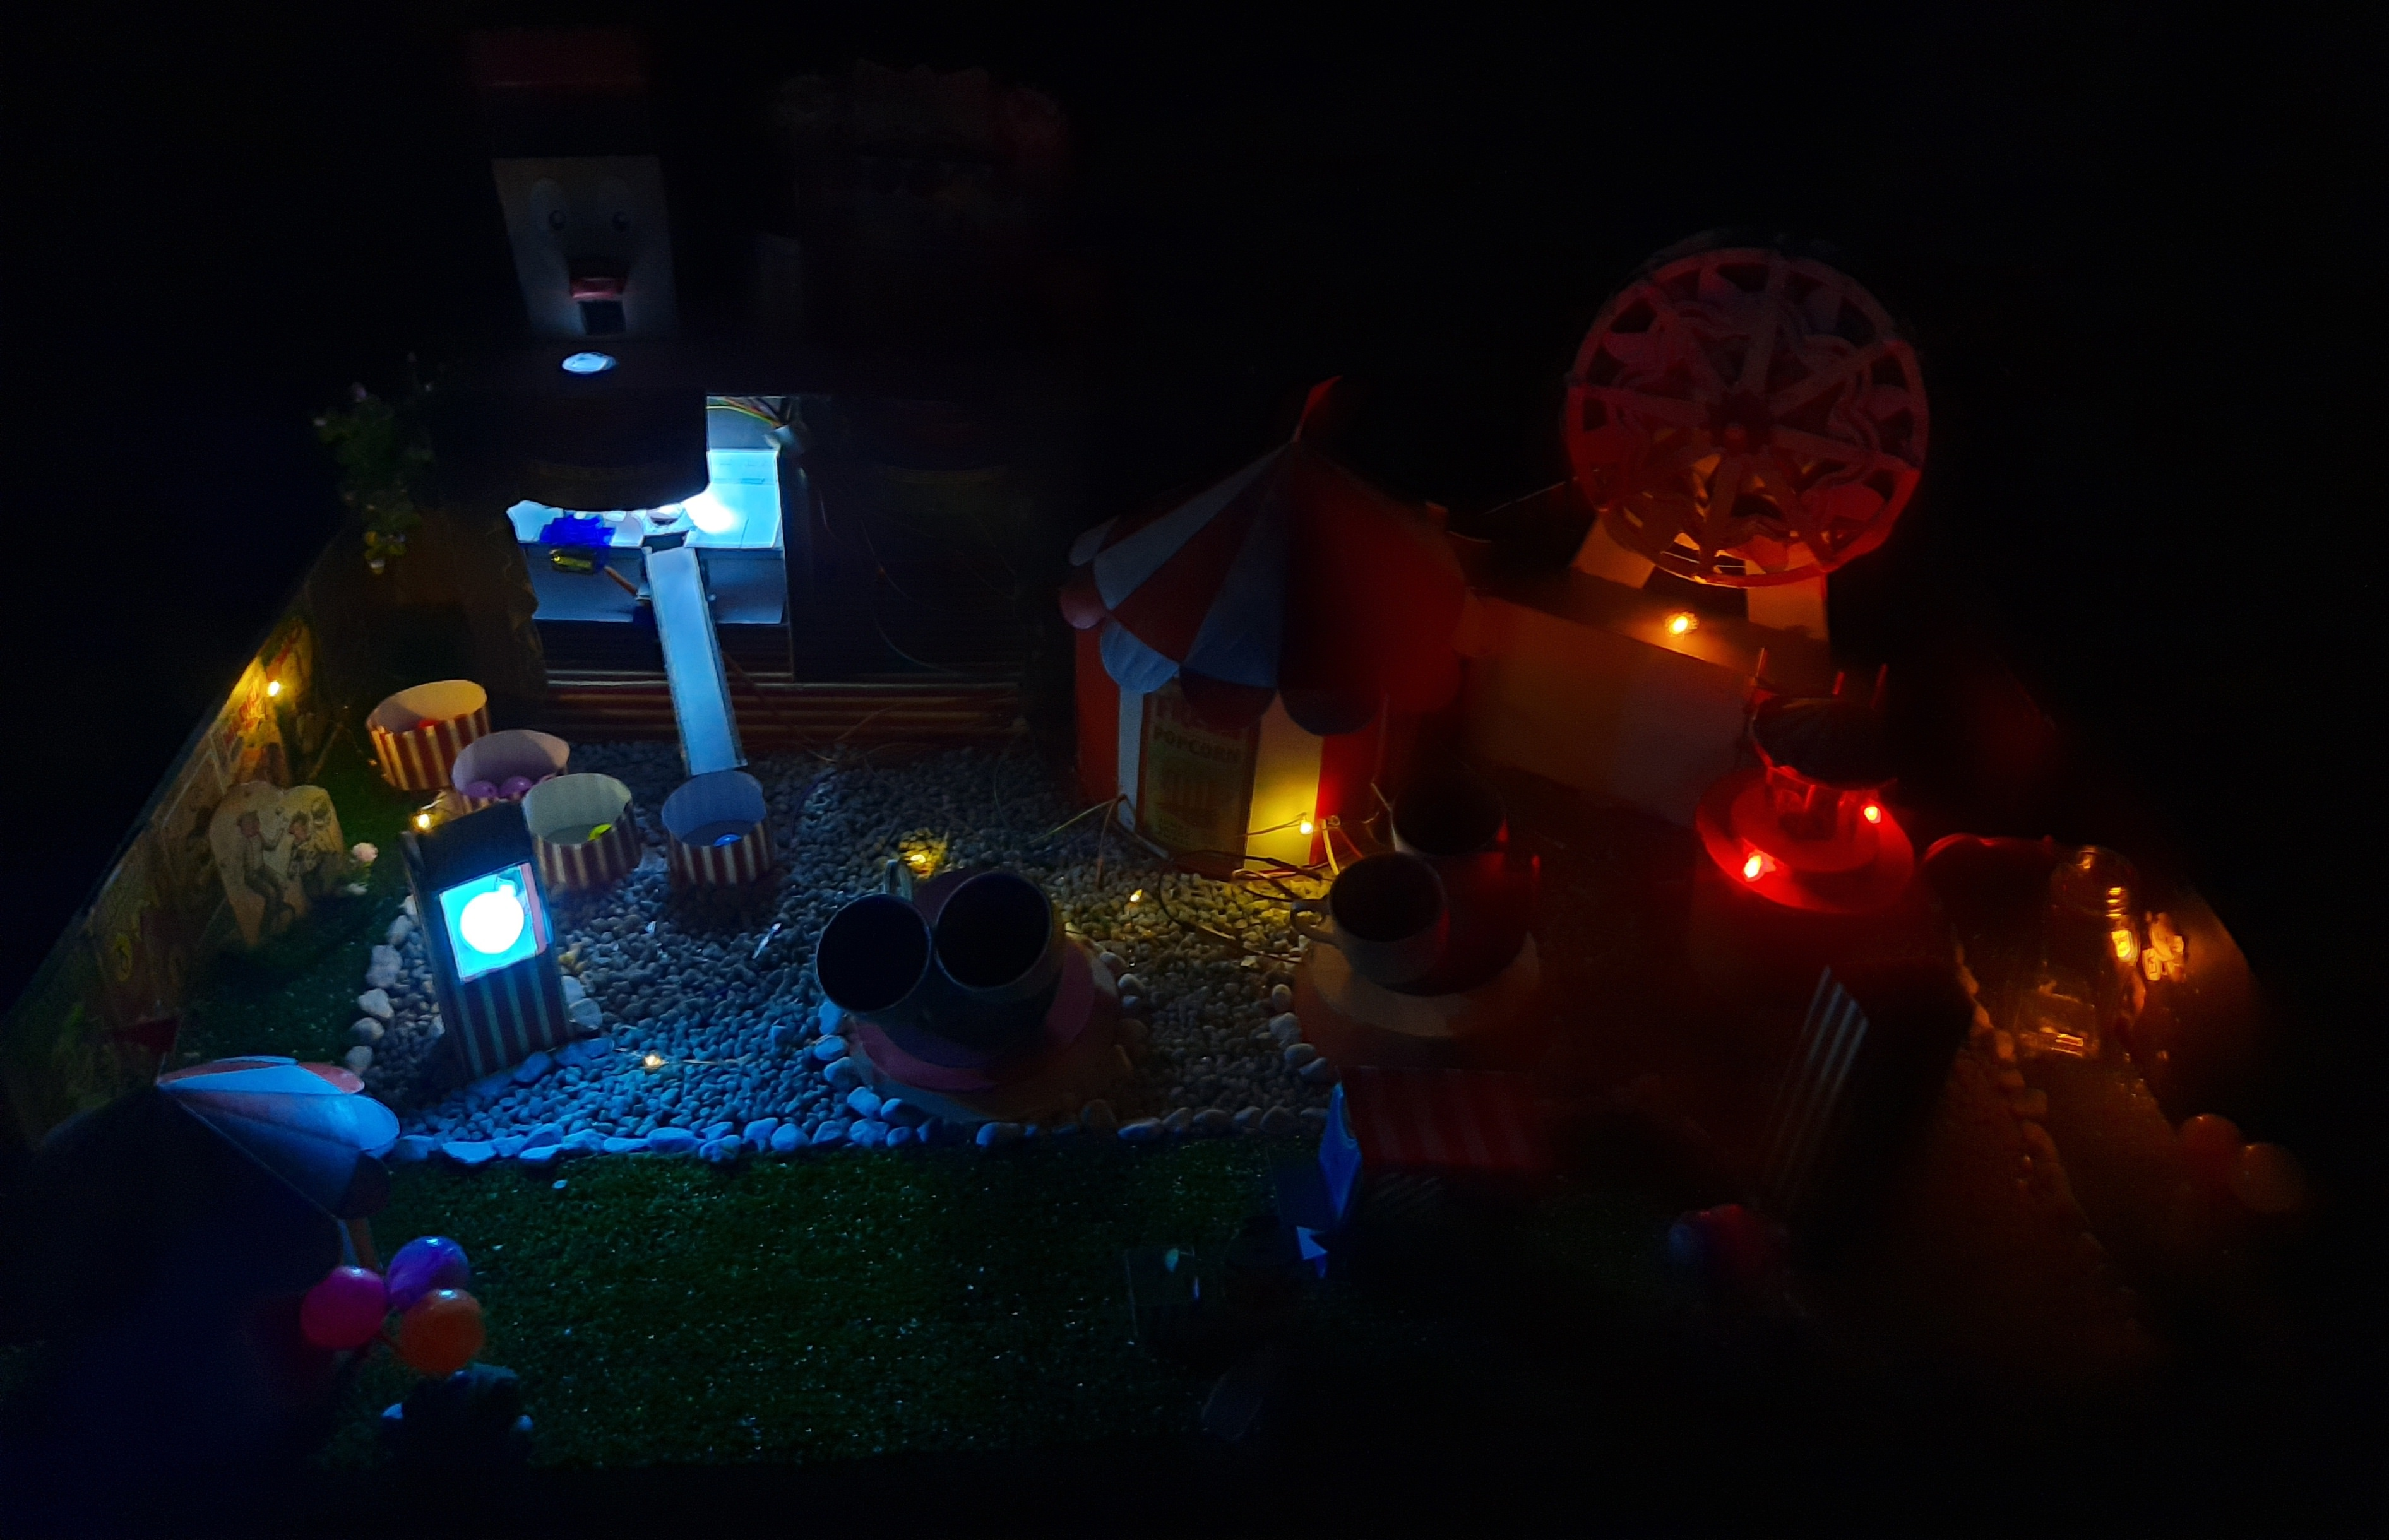
\includegraphics[width=0.7\textwidth]{svjetla}
  \caption{Osvjetljenje sistema}
  \label{fig:Slika_osvjetljenje}
\end{figure}

Drugi podsistem je igra, prikazana izbliza na slici \ref{fig:Slika_pod1}, u kojoj korisnik pogađa boju loptice koja izađe iz aparata. Prvo pusti lopticu da uđe u podsistem, odabere na mobitelu da će igrati igru, te onda pogađa boju loptice pritiskom push buttona, koji je smješten u dizajn igre ''pogodi balon'', koja često bude u zabavnim parkovima. Ako pogodi boju, zasvijetli zelena dioda, a ako promaši, zasvijeli crvena. Boja se čita senzorom za boju, a servo motorima se loptice prebacuju u određenu posudu. U posudama su loptice sortirane po boji.

Treći podsistem je vračara, također vidljiva na slici \ref{fig:Slika_pod1}, čija RGB dioda se uključuje se i isključuje po korisnikovoj želji uz pomoć aplikacije.

\begin{figure}[h!]
  \centering
  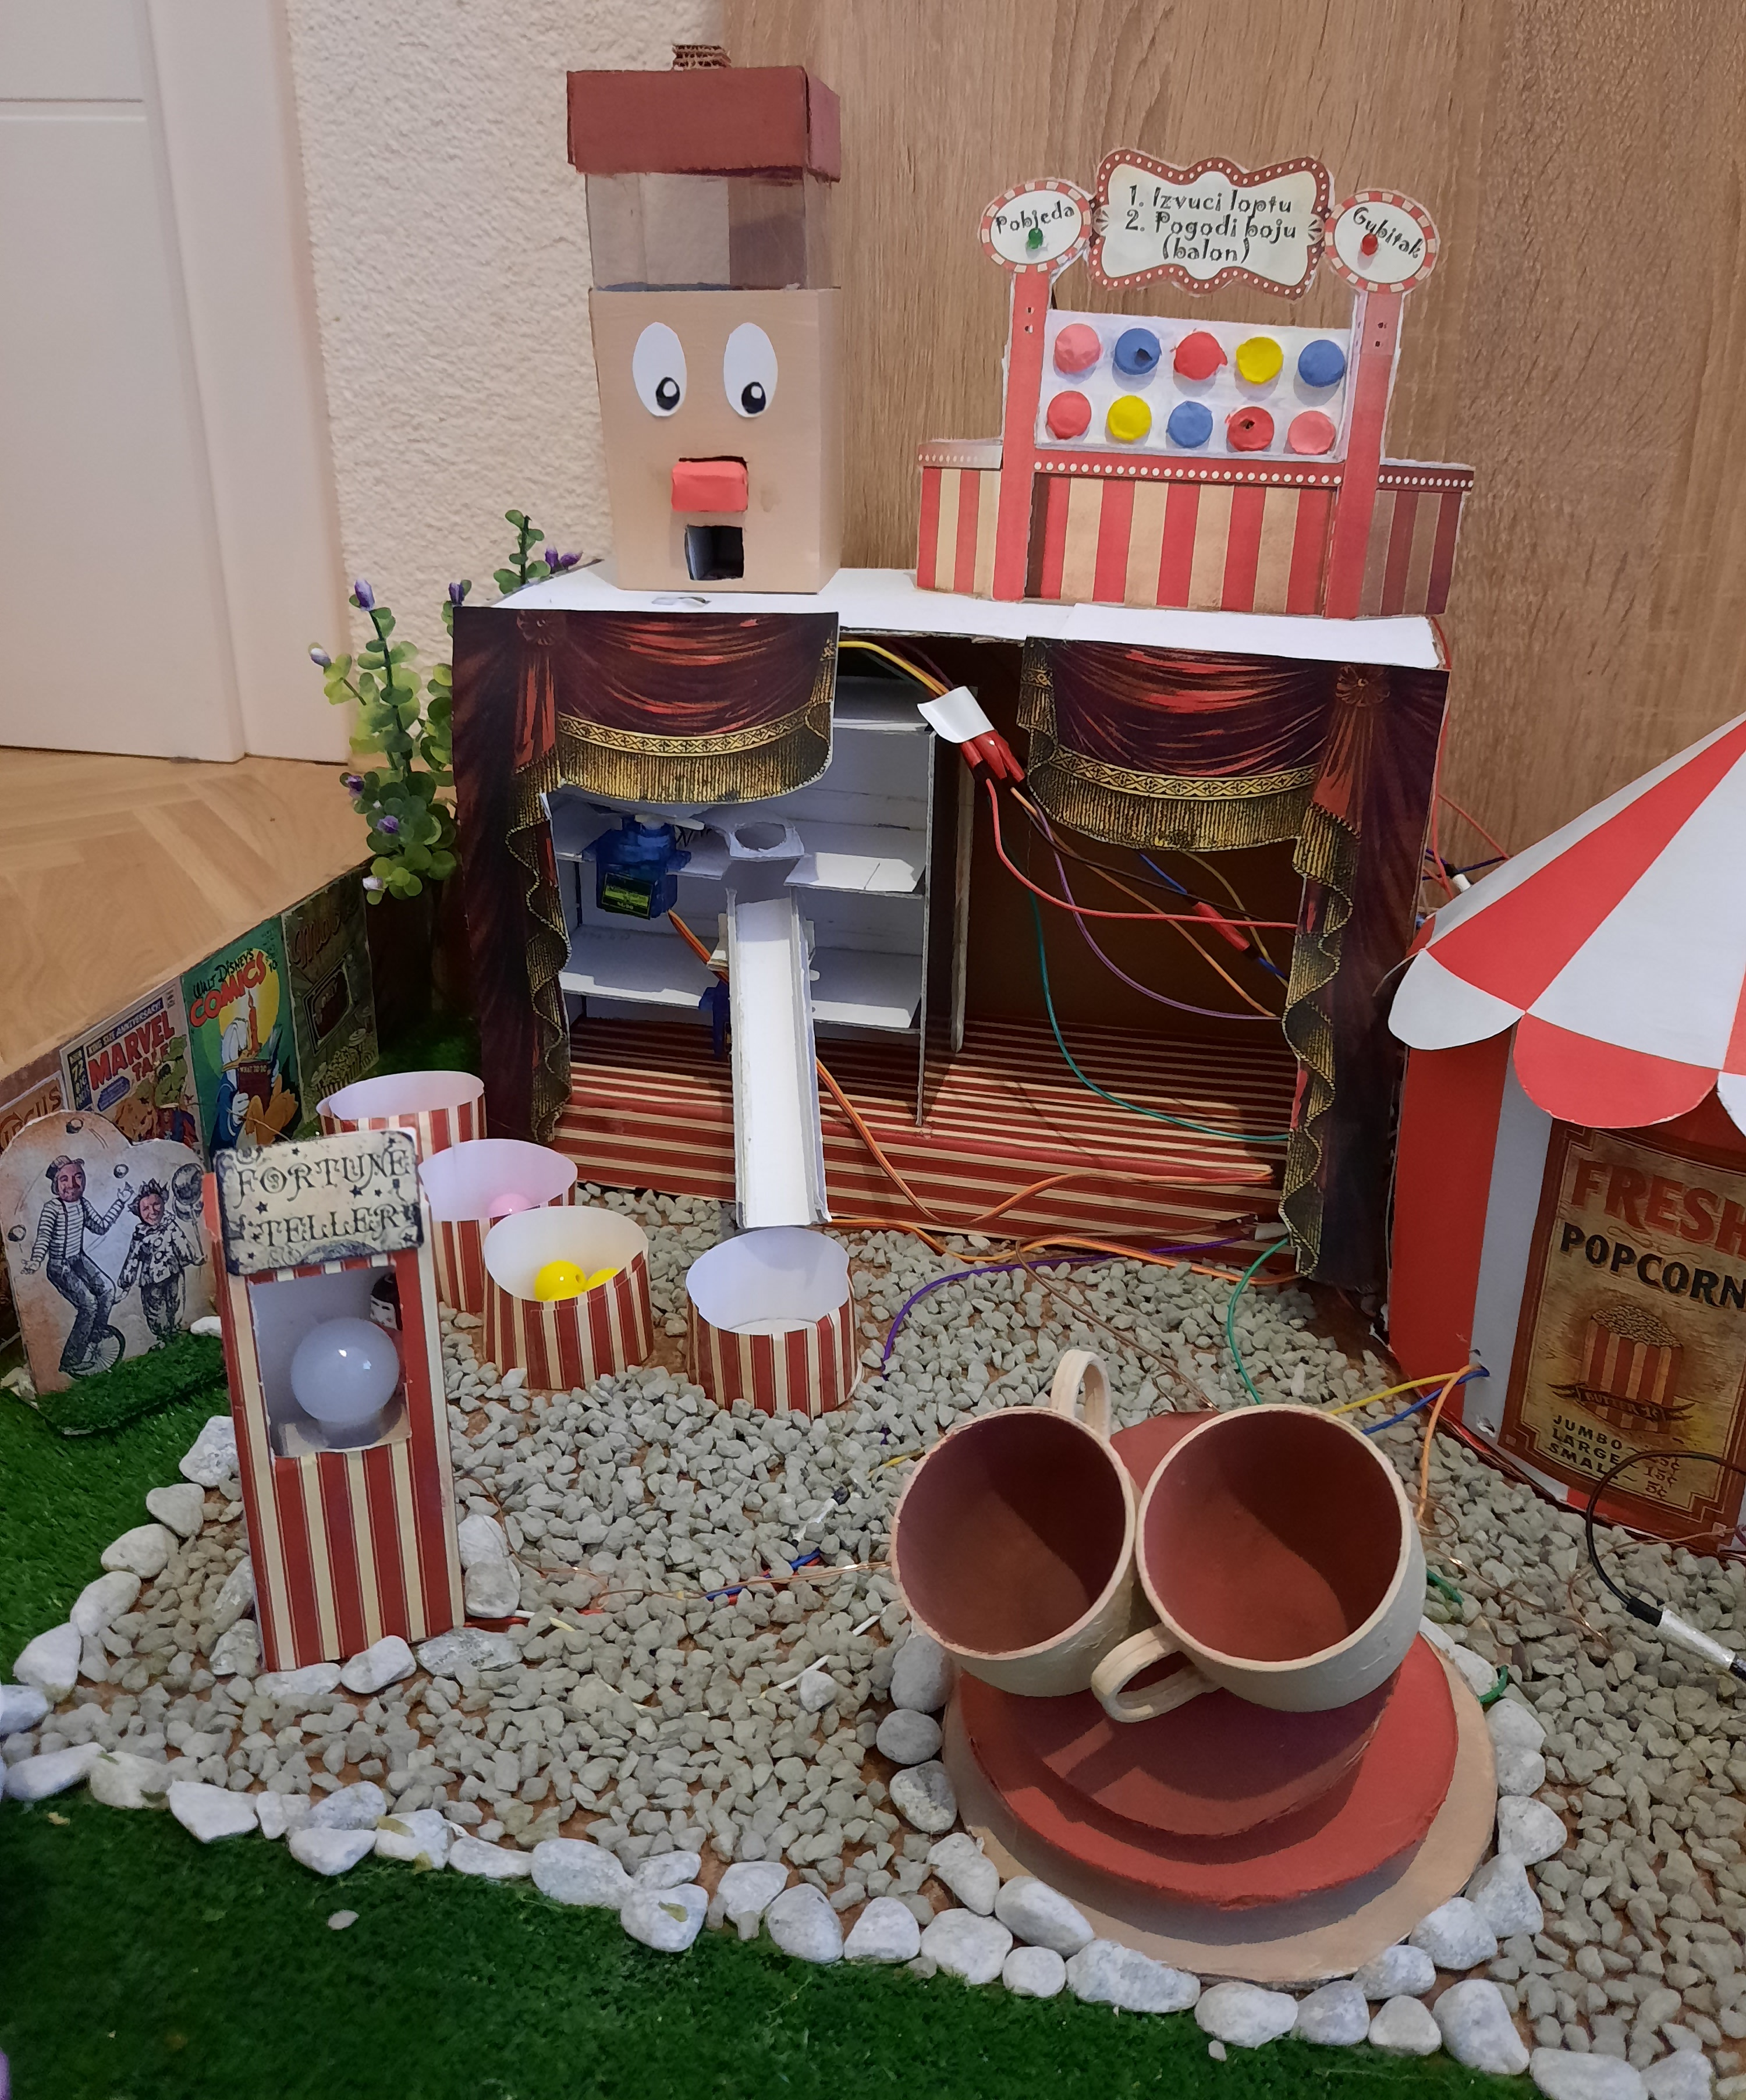
\includegraphics[width=0.5\textwidth]{pod1}
  \caption{Podsistemi igra i vračara}
  \label{fig:Slika_pod1}
\end{figure}

Četvrti podsistem je karusel, odnosno vrtuljak sa konjićima. Napravljen je od kartona po šablonu s Interneta. U sebi sadrži DC motor sa zupčanicima koji usporava njegovo okretanje kako ne bi bio prebrz. Pokreće se i zaustavlja po korisnikovoj želji uz pomoć aplikacije.

Peti podsistem je vrtuljak. Napravljen je od jako detaljnog šablona koji je preuzet s Interneta i modificiran kako bi odgovarao sistemu. Ima sjedala koja se mogu pomjerati. U njemu se nalazi jači DC motor, od 12 V, pošto ga slabiji ne mogu pokrenuti. Pokreće se i zaustavlja po korisnikovoj želji uz pomoć aplikacije.

Šesti podsistem su šoljice, koje se vrte uz pomoć DC motora ispod njih. Pokreću se i zaustavljaju po korisnikovoj želji uz pomoć aplikacije. Kako bi svi DC motori imali dovoljno snage da se pokrenu, samo za njih je osiguran ulazni napon od 6 baterija po 1,5 V, koji je puno bolji za DC motore od standardnih baterija od 9 V. 

\begin{figure}[h!]
  \centering
  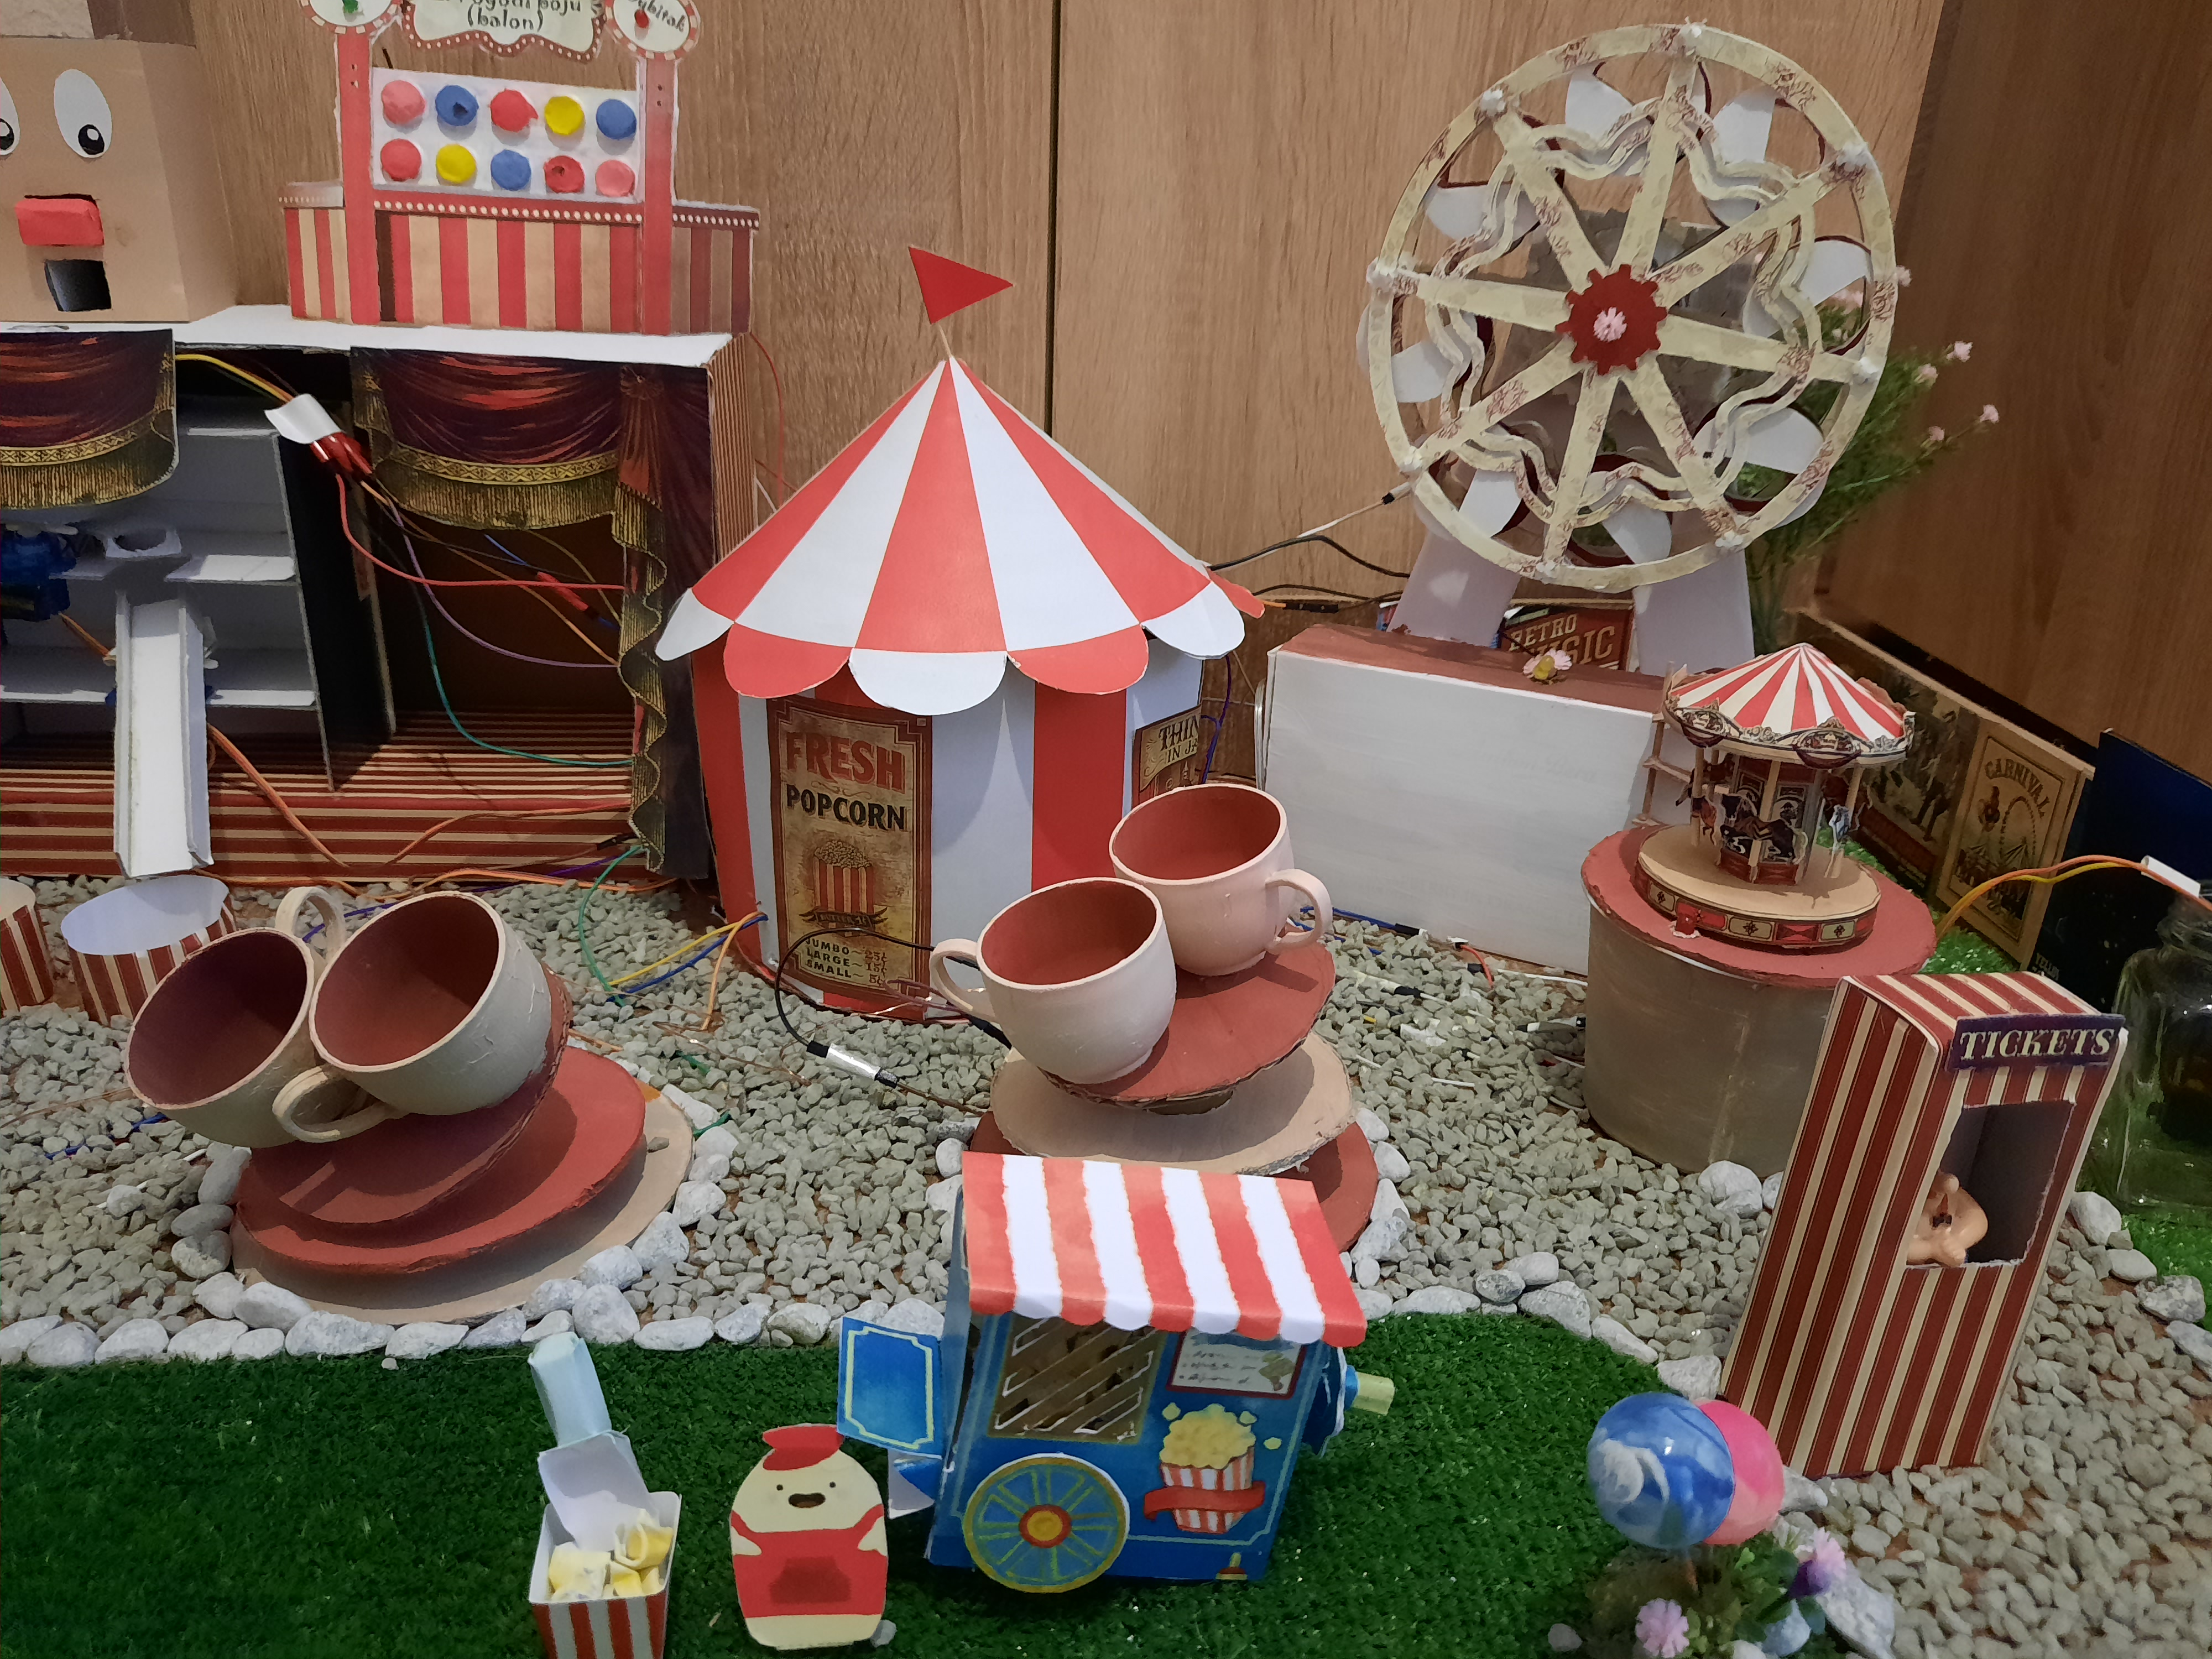
\includegraphics[width=0.7\textwidth]{pod2}
  \caption{Podsistemi  karusel, vrtuljak i šoljice}
  \label{fig:Slika_pod2}
\end{figure}

Sedmi podsistem je muzika koja se pušta s SD kartice preko zvučnika. SD kartica je morala biti povezana na posljednja 4 pina Arduino Mega pločice (prije 5 V pinova), pošto su to pinovi namijenjeni za asinhronu komunikaciju u kojoj je Arduino Mega pločica master element. Zvučnik je morao biti povezan na pin 5, 11 ili 46, inače ne bi radio. Pjesma za puštanje morala je biti konvertovana u .wav datoteku, sa frekvencijom 16 KHz, da bi zvuk bio neometano pušten. Pjesma se pokreće i zaustavlja po korisnikovoj želji uz pomoć aplikacije.

Svaki dio sistema prvotno je zasebno testiran, odnosno, sistem je rađen postepeno. Tek u završnoj fazi projektovanja sistema, svi su dijelovi sklopljeni u jednu cjelinu i usklađen je međusoban rad svih njegovih komponenti.

Motori koji pokreću određene dijelove prvo su testirani spajanjem direktno na napon, a tek onda povezani na modul, te na Arduino. Možda najzahtjevniji dio projektovanja sistema je bio usklađivanje napajanja, brzine vrtnje motora, te težine objekata koji se trebaju pokretati motorom. Kad je brzina motora premalena ili napon previše nizak, dijelovi se ne mogu vrtjeti, a prevelika brzina može oštetiti neki dio. Također, L298N driver za motore, jedini na lokalnom tržištu, nije savršen.

Rad sistema je jako teško prikazati na jednoj slici, puno bolji način je animacija ili video, s obzirom da se većina komponenti vrti, svijetli ili okreće, te se muzika sluša. 

 \begin{figure}[h!]
  \centering
  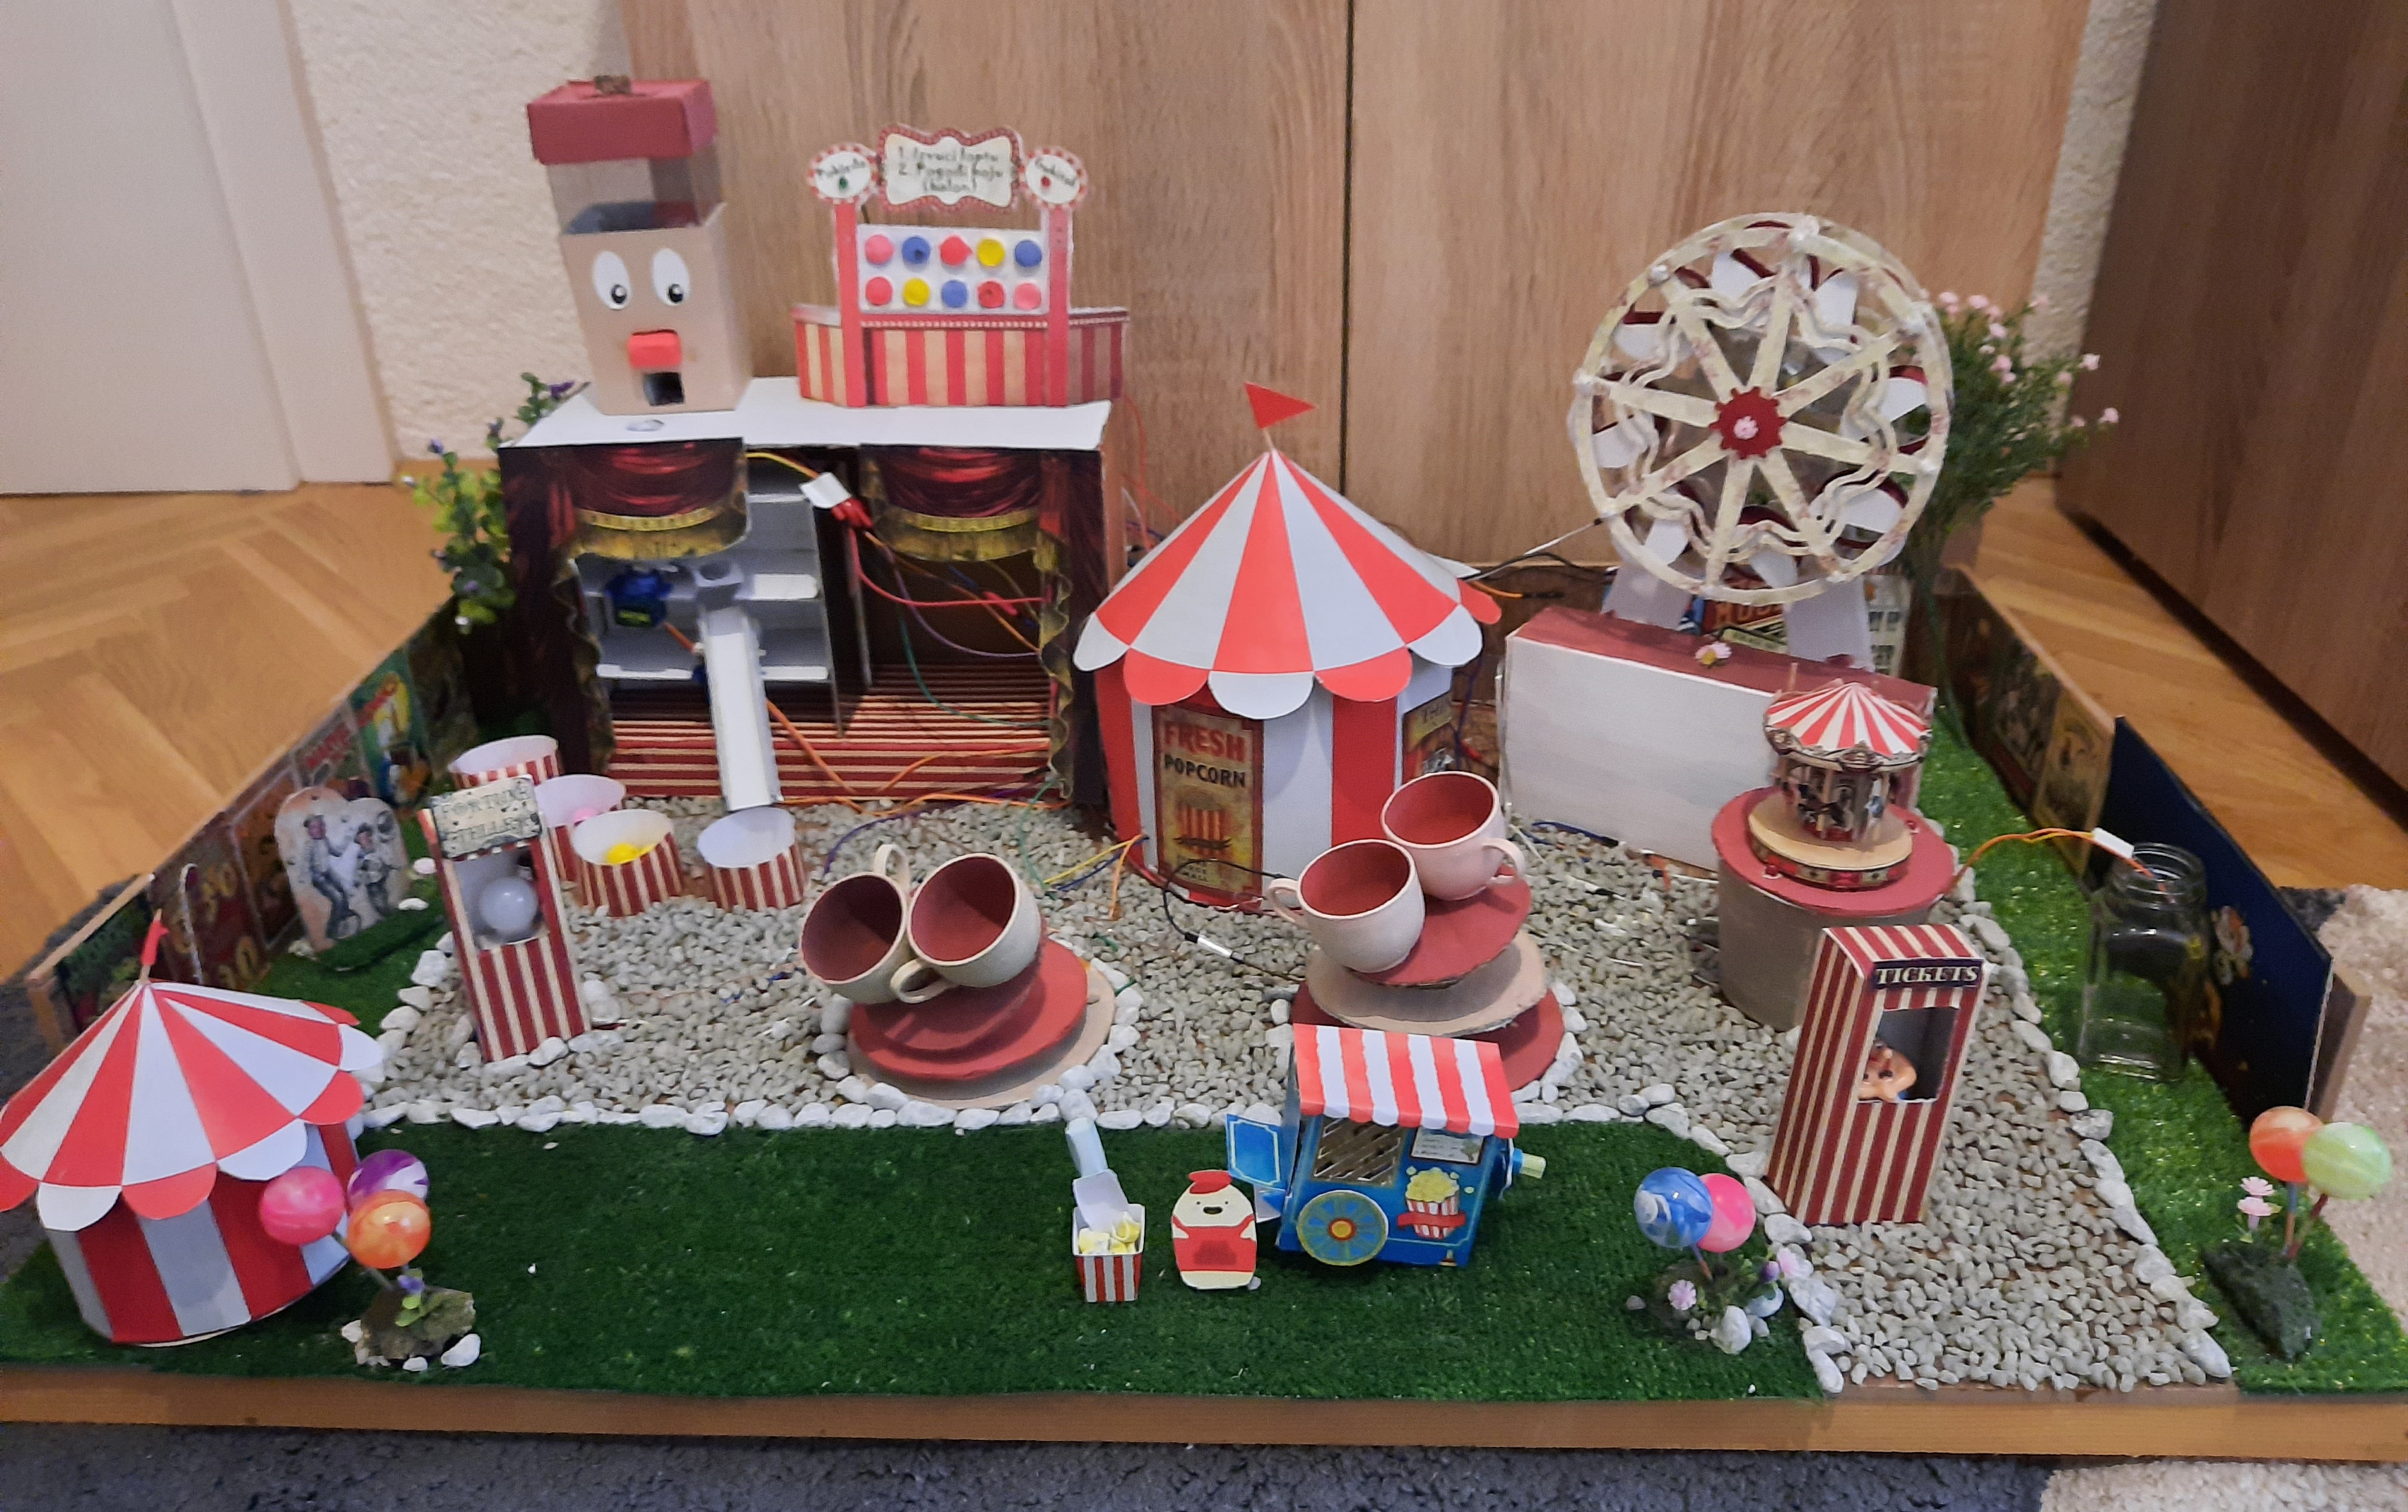
\includegraphics[width=0.7\textwidth]{maketa3}
  \caption{Maketa sistema}
  \label{fig:Slika_Maketa}
\end{figure}

Prednosti ovog sistema su da je potpuno jedinstven, stabilan, detaljan, te, zbog pozicioniranja USB kabla od Arduino pločice na lagano dohvatljivo mjesto, podložan nadogradnji i promjeni. Mane sistema su materijal, karton nije dobar materijal za gradnju, te nesavršenost komponenti.

%Zaključak
\chapter{Zaključak}

U ovom seminarskom radu prikazano je koji su to koraci potrebni za projektovanje jednog mikroproceskorskog sistema koji funkcioniše u realnom vremenu. Sistem koji je napravljen je lunapark. \\

Lunapark ili park zabave je ograđeni prostor sa nizom elemenata namijenjenih zabavi većeg broja ljudi, te zaradi vlasnika. Pojava određenih ograđenih prostora samo za zabavu postoji još od početka prošlog milenija, a smatra se da su moderni parkovi zabave nastali u 19. stoljeću. Danas su veoma popularni takozvani tematski parkovi, odnosno lunaparkovi koji su napravljeni na neku temu. \\

Za kreiranje ovog sistema, korištena je Arduino Mega pločica, velik broj komponenti, Arduino programsko okruženje, Android Studio programsko okruženje, te Tensorflow Lite neuronska mreža. Ukrasni, nefunkcionalni dio, pravljen je od kartona, te su slike uređivane uz pomoć Adobe Photoshopa. Dobijen je lijep i funkcionalan sistem, ali nesavršen zbog materijala - kartona, te nesavršenih komponenti. \\

Pokretanje sistema realizirano je kao sistem sa ulaznicama. Korisnik treba pokretnuti Android aplikaciju, te preko kamere izvršiti akviziciju slike. Ako je na slici jedna od ulaznica sistema, korisniku se dopušta da se poveže na bluetooth i upravlja pojedinim dijelovima sistema. Prepoznavanje ulaznice istrenirano je pomoću neuronske mreže. Radnje koje korisnik kontrolira su pokretanje i zaustavljanje vrteški, uključivanje i isključivanje svjetala, pokretanje igre, te pokretanje i zaustavljanje muzike. 







%%%%%%%%%%%%%%%%%%%%%%%%%%%%%%%%%%%%%%%%%%%%%%%%%%%%%%%%%%%%%%%%%%%%
%\backmatter
%%%%%%%%%%%%%%%%%%%% LISTA PUBLIKACIJA %%%%%%%%%%%%%%%%%%%%%%%%%%%%%
%\chapter*{Lista publikacija}
%\addcontentsline{toc}{chapter}{Lista publikacija}

%%%%%%%%%%%%%%%%%%%%%%% LITERATURA %%%%%%%%%%%%%%%%%%%%%%%%%%%%%%%%%
\addcontentsline{toc}{chapter}{Literatura}
\bibliographystyle{IEEEtranETF} 
\bibliography{literatura}

%%%%%%%%%%%%%%%%%%%%%%%%%%% INDEKS POJMOVA %%%%%%%%%%%%%%%%%%%%%%%%%
%\addcontentsline{toc}{chapter}{Indeks pojmova}
\printindex 

%%%%%%%%%%%%%%%%%%%%%%%%%%%%%%%%%%%%%%%%%%%%%%%%%%%%%%%%%%%%%%%%%%%%%%
%%%%%%%%%%%%%%%%%%%%%%%%% PRILOZI %%%%%%%%%%%%%%%%%%%%%%%%%%%%%%%%%%%%
%%%%%%%%%%%%%%%%%%%%%%%%%%%%%%%%%%%%%%%%%%%%%%%%%%%%%%%%%%%%%%%%%%%%%%
\begin{appendices}
%Priloge je najbolje raditi u odvojenim fajlovima
%Prilog 1
\chapter{Programski kôd}

Programski kôd korišten za rad sistema dan je u nastavku.
\begin{lstlisting}[frame=single,language=C++,numbers=left, numberstyle=\tiny, xleftmargin=0.05\textwidth, xrightmargin=0.05\textwidth, basicstyle=\ttfamily\footnotesize]
#include <Servo.h>
#include "SD.h"
#define SD_ChipSelectPin 53
#include "TMRpcm.h"
#include "SPI.h"

// SD kartica
TMRpcm tmrpcm;
// Senzor za boju
#define S0 2
#define S1 3
#define S2 4
#define S3 5
#define sensorOut 6
const int crveniButton = 28;    
const int plaviButton = 26; 
Servo gornjiServo;
Servo donjiServo;

// svjetla
const int crvenaDioda = 29; 
const int zelenaDioda = 30; 

const int dioda1 = 32; 
const int dioda2 = 31; 
const int dioda3 = 33;
const int dioda4 = 34;
const int svjetla = 36;

// aplikacija
long int data;

// motori
#define enA 10
int motor1pin1 = 40;
int motor1pin2 = 41;

int motor2pin1 = 42;
int motor2pin2 = 43;

int motor3pin1 = 44;
int motor3pin2 = 45;

int motor4pin1 = 46;
int motor4pin2 = 47;

// vracara
int crveni_pin= 11;
int zeleni_pin = 12;
int plavi_pin = 13;

// senzor za boju
int frekvencija = 0;
int color = 0;
int crveniButtonState = 0;    
int plaviButtonState = 0; 
// citanje buttona

void setup(){
// pokretanje SD kartice
tmrpcm.speakerPin = 46;
Serial.begin(9600);
if(!SD.begin(SD_ChipSelectPin)){
  Serial.println("SD fail");
  return;
}
tmrpcm.setVolume(6);
    
//bluetooth pokretanje na serijskom portu 1
Serial1.begin(9600);

// senzor za boju
pinMode(crveniButton, INPUT);
pinMode(plaviButton, INPUT);
pinMode(zutiButton, INPUT);
pinMode(S0, OUTPUT);
pinMode(S1, OUTPUT);
pinMode(S2, OUTPUT);
pinMode(S3, OUTPUT);
pinMode(sensorOut, INPUT);

// skaliranje
digitalWrite(S0, HIGH);
digitalWrite(S1, LOW);

gornjiServo.attach(22);
donjiServo.attach(24);

// motori
 pinMode(motor1pin1, OUTPUT);
 pinMode(motor1pin2, OUTPUT);
 pinMode(motor2pin1, OUTPUT);
 pinMode(motor2pin2, OUTPUT);
 pinMode(motor3pin1, OUTPUT);
 pinMode(motor3pin2, OUTPUT);
 pinMode(motor4pin1, OUTPUT);
 pinMode(motor4pin2, OUTPUT);

// vracara
pinMode(crveni_pin, OUTPUT);
pinMode(zeleni_pin, OUTPUT);
pinMode(plavi_pin, OUTPUT);
 
// DIODE
pinMode(zelenaDioda, OUTPUT);
pinMode(crvenaDioda, OUTPUT);
pinMode(dioda1, OUTPUT);
pinMode(dioda2, OUTPUT);
pinMode(dioda3, OUTPUT);
pinMode(dioda4, OUTPUT);
pinMode(svjetla, OUTPUT);
    
void loop(){
 
while(Serial1.available()==0) ;

donjiServo.write(0);
if(Serial1.available()>0) {
data = Serial1.parseInt();
 
} 

delay(400);
Serial.print(data);
 
if (data == 67){
  diodePali();
}
if (data == 76){
  diodeGasi();
}
if (data == 23){
  vracara();
}
if (data == 32){
  vracaraUgasi();
}
if (data == 56){
  analogWrite(enA, 160); 
  digitalWrite(motor4pin1, HIGH);
  digitalWrite(motor4pin2, LOW);
}
if (data == 65){
  digitalWrite(motor4pin1, LOW);
  digitalWrite(motor4pin2, LOW);
}
if (data == 34){
  digitalWrite(motor1pin1, LOW);
  digitalWrite(motor1pin2, HIGH);
}
if (data == 43){
  digitalWrite(motor1pin1, LOW);
  digitalWrite(motor1pin2, LOW);
}
if (data == 11){ 
  digitalWrite(motor3pin1, HIGH);
  digitalWrite(motor3pin2, LOW);
  digitalWrite(motor2pin1, LOW);
  digitalWrite(motor2pin2, HIGH);
}
if (data == 21){
  digitalWrite(motor3pin1, LOW);
  digitalWrite(motor3pin2, LOW);
  digitalWrite(motor2pin1, LOW);
  digitalWrite(motor2pin2, LOW);
}
if (data == 91){ 
   tmrpcm.play("test.wav");
}
if (data == 19){
   tmrpcm.pause();
}
if (data == 89){ 
   crveniButtonState = digitalRead(crveniButton);
   plaviButtonState = digitalRead(plaviButton);

if (crveniButtonState == HIGH || zutiButtonState == HIGH || plaviButtonState == HIGH) {
    senzorZaBoje(crveniButtonState, zutiButtonState, plaviButtonState);
}
}
if (data == 98){
   donjiServo.write(110);
}
if (data == 99){ 
   crveniButtonState = digitalRead(crveniButton);
   plaviButtonState = digitalRead(plaviButton);

if (crveniButtonState == HIGH || zutiButtonState == HIGH || plaviButtonState == HIGH) {
    senzorZaBoje(crveniButtonState, zutiButtonState, plaviButtonState);
}
 diodePali();
   digitalWrite(motor1pin1, LOW);
   digitalWrite(motor1pin2, HIGH);
  digitalWrite(motor3pin1, HIGH);
  digitalWrite(motor3pin2, LOW);
  digitalWrite(motor2pin1, LOW);
  digitalWrite(motor2pin2, HIGH);
  analogWrite(enA, 160); 
  digitalWrite(motor4pin1, HIGH);
  digitalWrite(motor4pin2, LOW);
  vracara();
  tmrpcm.play("test.wav");
}
if (data == 88){
  diodeGasi();
  donjiServo.write(110);
  digitalWrite(motor1pin1, LOW);
  digitalWrite(motor1pin2, LOW);
  digitalWrite(motor3pin1, LOW);
  digitalWrite(motor3pin2, LOW);
  digitalWrite(motor2pin1, LOW);
  digitalWrite(motor2pin2, LOW);
  analogWrite(enA, 160); 
  digitalWrite(motor4pin1, LOW);
  digitalWrite(motor4pin2, LOW);
  vracaraUgasi();
  tmrpcm.pause();
}

}
void vracara(){
  RGB_color(255, 0, 0); // crvena
  delay(1000);
  RGB_color(0, 255, 0); // zelena
  delay(1000);
  RGB_color(0, 0, 255); // plava
  delay(1000);
  RGB_color(255, 255, 125); // roza
  delay(1000);
  RGB_color(0, 255, 255); // cijan
  delay(1000);
  RGB_color(255, 0, 255); // magenta
  delay(1000);
  RGB_color(255, 255, 0); // zuta
  delay(1000);
  RGB_color(255, 255, 255); // bijela
  delay(1000);
}


void RGB_color(int crvena, int zelena, int plava) {
  analogWrite(crveni_pin, crvena);
  analogWrite(zeleni_pin, zelena);
  analogWrite(plavi_pin, plava);
}

int readColor() {
// Citanje crvenih fotodioda
  digitalWrite(S2, LOW);
  digitalWrite(S3, LOW);
  frekvencija = pulseIn(sensorOut, LOW);
  int R = frekvencija;
    delay(50);

// Citanje zelenih fotodioda
  digitalWrite(S2, HIGH);
  digitalWrite(S3, HIGH);
  frekvencija = pulseIn(sensorOut, LOW);
  int G = frekvencija;
  delay(50);
  
// Citanje plavih
  digitalWrite(S2, LOW);
  digitalWrite(S3, HIGH);
  frekvencija = pulseIn(sensorOut, LOW);
  int B = frekvencja;
  delay(50);

  if((R<45 & R>32 & G<70 & G>50) || (R>70 & G<10 & B <50 & B>30) ){
    color = 1; // Crvena
  }
  if(R<45 & R>35 & B<40 &B>30){
    color = 2; // Roza
  }
  if(R<63 & R>50 & G<55 & G>45 & B<40 & B>29){
    color = 3; // Plava
  }
  if(R<40 & R>30 & G<50 & G>40 & B<46 & B>38){
    color = 4; // Zuta
  }
  return color;  
}

void senzorZaBoje(){
   crveniButtonState = digitalRead(crveniButton);
   plaviButtonState = digitalRead(plaviButton);

// Ako je pritisnut jedan od buttona, pokrese se dio programa. Ako korisnik pritisne odgovarajuci button, te pogodi koje je boje loptica, on pobijedi, pali se zelena dioda, u suprotnom, pali se crvena.
  if (crveniButtonState == HIGH || plaviButtonState == HIGH) {
  gornjiServo.write(120);
  delay(3000);
  
  for(int i = 115; i > 55; i--) {
    gornjiServo.write(i);
    delay(2);
  }
  delay(1000);
  
  color = readColor();
  color = readColor();
  color = readColor();
  color = readColor();
  
  delay(1000);  
   switch (color) {
    case 1: //crvena
    if (crveniButtonState == HIGH){
      digitalWrite(zelenaDioda, HIGH);
      digitalWrite(crvenaDioda, LOW);
    }
    if (plaviButtonState == HIGH ){
      digitalWrite(crvenaDioda, HIGH);
      digitalWrite(zelenaDioda, LOW);
    }
    donjiServo.write(50);
    break;
    case 2: //roza
    digitalWrite(crvenaDioda, HIGH);
    digitalWrite(zelenaDioda, LOW);
    donjiServo.write(75);
    break;
    case 3: // zuta
      digitalWrite(crvenaDioda, HIGH);
      digitalWrite(zelenaDioda, LOW);
    donjiServo.write(100);
    break;
    case 4: // plava
     if (plaviButtonState == HIGH){
    digitalWrite(zelenaDioda, HIGH);
    digitalWrite(crvenaDioda, LOW);
    }
    if (crveniButtonState == HIGH ){
    digitalWrite(crvenaDioda, HIGH);
    digitalWrite(zelenaDioda, LOW);
    }
    donjiServo.write(125);
    break;  
    case 0:
    break;
  }
  delay(300);
  
  for(int i = 55; i > 20; i--) {
    gornjiServo.write(i);
    delay(2);
  } 
  delay(500);
  
  for(int i = 29; i < 115; i++) {
    gornjiServo.write(i);
    delay(2);
  }
  color=0;
  }
}

void vrtiMotore(){
  digitalWrite(motor1pin1, HIGH);
  digitalWrite(motor1pin2, LOW);

  digitalWrite(motor2pin1, HIGH);
  digitalWrite(motor2pin2, LOW);

  digitalWrite(motor3pin1, HIGH);
  digitalWrite(motor3pin2, LOW);
  
    analogWrite(enA, 160);  // upravljanje brzinom
  digitalWrite(motor4pin1, HIGH);
  digitalWrite(motor4pin2, LOW);
}
 \end{lstlisting}
\end{appendices}

\end{document}
